\chapter{Exactly solvable models of nuclei}
精确可解的模型在核的壳模型发展中扮演了重要的作用,促进我们对原子核配对性质的理解以及在几何和代数模型的背景下对集体核现象的描述。本文综述了核的精确可解模型,重点讨论了概念问题而非技术问题。
\section{Introduction}
原子核是一个多体系统,主要受复杂和有效的 in-mideum 相互作用所控制,因此具有丰富的谱学性质。这些效应包括闭合壳层附近核子的独立运动,关联的两核子对的形成,以及由许多核子的协同运动引起的振动和转动的集体效应。目前对所观察到的各种核激发态的理论描述有两种可能的微观方法作为出发点。自洽平均场方法从一个给定的核子的有效相互作用或能量泛函开始来构造平均核子场;这导致了我们对集体模型的描述是从构成一个给定核子的所有中子和质子之间的相互关联来开始的。另一方面,球形核壳模型包含了在某种封闭壳结构外中子和质子的所有可能的相互作用。这两种方法都使用数值算法,因此是计算密集型的。

本文综述了这两种方法中能被精确地求解的一类子模型,并在此过程中强调了与原子核中成对关联系统的性质以及集体运动模式有关的一些一般结果。完全可解的模型必须具有图解性质,虽然仅对特定的核有效。但它们可以作为使用数值方法建立更真实的模型研究核素图大区域(同位素系列或同中子素系列)数据的参考或“基准”。这里的重点是精确可解模型本身,而不是与数据的比较。本文最后提到的几本书讨论了精确可解模型的后一个方面。

\section{An algebraic formulation of the quantal $n$-body problem}
对称性分析和代数方法不局限于核物理中的某些模型,而是可以普遍应用于寻找量子$n-$体问题的特殊解。这一部分将对此进行解释。

为了描述非相对论量子力学中$n-$体系统的定态性质,需要求解与时间无关的薛定谔方程:
\begin{equation}\label{eq_schrodinger}
\hat{H}\Psi(\varepsilon_1,\cdot,\varepsilon_n)=E\Psi(\varepsilon_1,\cdots,\varepsilon_n)
\end{equation}
其中$H$是多体系统的哈密顿量
\begin{equation}\label{eq_hamilt}
\hat{H}=\sum_{k=1}^n\left(\frac{\hat{p}^2_k}{2m_k}+\hat{V}_1(\varepsilon_k)\right)+\sum_{k<l}\hat{V}_2(\varepsilon_k,\varepsilon_l)+\sum_{k<l<m}\hat{V}_3(\varepsilon_k,\varepsilon_l,\varepsilon_m)+\cdots
\end{equation}
其中$m_k$和$\hat{p}_k^2/2m_k$分别是第$k$个粒子的质量和动能。这些粒子可以是玻色子或费米子。它们可能携带一个本征自旋和/或具有其他本征变量的特征(例如同位旋,其投影可以区分中子和质子)。这些粒子的变量$k$,以及他们的坐标变量$\bm{r}_k$,整体的被标记为$\varepsilon_k$。除了动能和一个可能的外部势场$\hat{V}_1(\varepsilon_k)$外,哈密顿量\ref{eq_hamilt}还包含代表组成粒子之间的两体、三体以及可能的多体相互作用项。$n-$体量子系统的定态性质通过在满足额外的玻色子交换对称和费米子交换反对称的限制下,求解薛定谔方程方程\ref{eq_schrodinger}来决定。

哈密顿量\ref{eq_hamilt}可以在二次量子化的情况下等效的写出来。其单体部分描述了一个独立的无相互作用的粒子体系,定义了一个由单粒子态$\phi_\alpha(\varepsilon_k)$构成的基,其中$\alpha$标记了一个在势场$\hat{V}_1$下的定态。在狄拉克符号系统下,这个单粒子态可以写成$\left<\varepsilon|\alpha\right>$,其中右矢$\left|\alpha\right>$可以利用产生算符$c_\alpha^\dag$作用在真空态上得到,$\left|\alpha\right>=c_\alpha^\dag\left|\textrm{o}\right>$。厄密伴随左矢也可以类似的利用湮灭算符$c_\alpha$,$\left<\alpha\right|=\left<\textrm{o}\right|c_\alpha$。一个多体系统的态现在可以简写为$\left|\alpha\beta\cdots\right>=c_\alpha^\dag c_\beta^\dag\cdots\left|\textrm{o}\right>$,而Pauli原理是自动满足的,当产生和湮灭算符$c_\alpha^\dag$、$c_\alpha$,在粒子是玻色子和费米子时分别满足对易关系和反对易关系,即
\begin{equation*}
[c_\alpha,c_\beta^\dag]=\delta_{\alpha\beta},\quad[c_\alpha,c_\beta]=[c_\alpha^\dag,c_\beta^\dag]=0
\end{equation*}
或者
\begin{equation*}
\{c_\alpha,c_\beta^\dag\}=\delta_{\alpha\beta},\quad\{c_\alpha,c_\beta\}=\{c_\alpha^\dag,c_\beta^\dag\}=0
\end{equation*}
根据前面的定义,哈密顿量\ref{eq_hamilt}可以重新写为
\begin{equation}\label{eq_halmiton}
\hat{H}=\sum_\alpha\varepsilon_\alpha c_\alpha^\dag c_\alpha+\sum_{\alpha\beta\gamma\delta}v_{\alpha\beta\gamma\delta}c_\alpha^\dag c_\beta^\dag c_\gamma c_\delta+\cdots
\end{equation}
其中$\varepsilon_\alpha$是与哈密顿量\ref{eq_hamilt}中的单体项相关的系数,$v_{\alpha\beta\gamma\delta}$是与两体相互作用相关的系数,以此类推。求和是在单粒子态的整个完备集上的,在大多数应用中是无穷的。即使是在一组有限的单粒子态上求和,薛定谔方程的求解仍然是一项艰巨的任务,因为随着粒子数和可能的单粒子态的增加,多体态的Hilbert空间的维数是指数增长的。

与哈密顿量\ref{eq_halmiton}相关的薛定谔方程只有当粒子间无相互作用时才有直接解。在这种情况下,$n-$体问题变成了$n$个单体问题,使得这$n$个粒子的本征态变成了,当粒子是玻色子是是Slater恒等式,当粒子是费米子时是Slater行列式,即,本征态是$c_{\alpha_1}^\dag\cdots c_{\alpha_1}^\dag\left|\textrm{o}\right>$的形式。Slater恒等式或行列式是Hartree(-Fock)理论提出的一个重要的概念。虽然平均势或平均场方法隐式的包含相关性,但是Hartree(-Fock)理论理论并未明确地处理两体和多体的相互作用,但是Slater恒等式或行列式确实提供了一个可以对角化粒子间相互作用的基。阻止人们进行这种对角线化的主要障碍是基的维数。因此,问题在于相互作用是否可以绕过对角化,并且可以被解析的处理。

用对称性分析求解特定种类的哈密顿量\ref{eq_halmiton}的测量,是当发现它们可以用算符$\hat{u}_{\alpha\beta}\equiv c_{\alpha}^\dag c_\beta$来重新表述时开始的。后一种算符对于玻色子和费米子都可以证明服从下列交换关系:
\begin{equation}\label{eq_commu}
[\hat{u}_{\alpha\beta},\hat{u}_{\alpha'\beta'}]=\hat{u}_{\alpha\beta'}\delta_{\alpha'\beta}-\hat{u}_{\alpha'\beta}\delta_{\alpha\beta'}
\end{equation}
这表明$\hat{u}_{\alpha\beta}$生成酉李代数$U(\Omega)$,其中$\Omega$是单粒子基的维数。[在对易关系\ref{eq_commu}中,假定所有的指数都是指费米子或玻色子。而对于玻色子和费米子混合的情况将在后面单独处理。]代数$U(\Omega)$是这个问题的动力学代数$G_\textrm{dyn}$,在这个意义上,哈密顿量和其他算符都可以用它的生成元来表示。这不是哈密顿量的一个真正的对称性而是破缺的一个。与$G_\textrm{dyn}$相关的对称性的破缺是以一种特殊的方式进行的,这种方式可以方便地用一系列嵌套李代数来概括
\begin{equation}\label{eq_classi}
G_1\equiv G_\textrm{dyn}\supset G_2\supset\cdots\supset G_s\equiv G_\textrm{sym}
\end{equation}
其中,在嵌套中的最后的代数$G_\textrm{sym}=\textrm{SO}(3)$是真实对称性的代数,其生成元与哈密顿量对易。例。如,如果哈密顿量是转动不变的,那么其对称性代数是在三维转动的代数中的,$G_\textrm{sym}=\textrm{SO}(3)$。

为了理解分类\ref{eq_classi}在与多体哈密顿量\ref{eq_halmiton}的联系中的相关性,应该注意到,对于一个特定的嵌套代数链,应该对应于一类可以写成与链中的代数相关联的Casimir算子的线性组合哈密顿量,
\begin{equation}\label{eq_rew}
\hat{H}_\textrm{DS}=\sum_{r=1}^s\sum_m\kappa_{rm}\hat{C}_m[G_r]
\end{equation}
其中,$\kappa_{rm}$是任意的系数。$\hat{C}_m[G_r]$即是代数$G_r$的所谓的 Casimir 算符;他们可以被写为$G_r$的生成元的直到$m$阶乘积的线性组合,并且满足与$G_r$的所有的生成元对易的重要性质,对于所有的$\hat{g}\in G_r$满足$[\hat{C}_m[G_r],\hat{g}]=0$。在公式\ref{eq_rew}中的 Casimir 算符满足$[\hat{C}_m[G_r],\hat{C}_{m'}[G_{r'}]]=0$,即他们都相互对易。这个性质可以由$G_r$的一个嵌套代数链的的所有元素都在$G_{r'}$中,反之亦然的这一个事实来证实。因此,哈密顿量\ref{eq_rew}被写成了对易算符的和,其本征态可以用与这些算符相关的量子数标记。注意,公式\ref{eq_classi}中的代数嵌套的条件对于构造一组交换算子,从而获得解析解是至关重要的。Casimir 算符可以通过算符$\hat{u}_{\alpha\beta}$的项表示,所以展开式\ref{eq_rew}在粒子中可以重写为公式\ref{eq_halmiton}的形式,其中相互作用的阶由不变量的最高阶决定。

总而言之,哈密顿量\ref{eq_rew},其可以通过更一般的哈密顿量$\ref{eq_halmiton}$选择特殊的系数$\varepsilon_\alpha,v_{\alpha\beta\gamma\delta}$来得到,并且可以被解析求解。其本征态可以量子数$\Gamma_r$来表示,其表征出现在约化$\ref{eq_classi}$中的不同代数的不可约表示,从而得出可以方便地求和的如下的分类:
\begin{equation*}
{\setlength\arraycolsep{3pt}\renewcommand{\arraystretch}{0.7}
\begin{array}{ccccccc}
G_1&\supset&G_2&\supset&\cdots&\supset&G_s\\
\downarrow& &\downarrow& & & &\downarrow\\
\Gamma_1& &\Gamma_2& & & &\Gamma_s
\end{array}}
\end{equation*}
用解析方法求解得到的与哈密顿量\ref{eq_rew}有关的久期方程
\begin{equation*}
\hat{H}_\textrm{DS}\left|\Gamma_1\Gamma_2\cdots\Gamma_s\right>=\sum_{r=1}^s\sum_m\kappa_{rm}E_m(\Gamma_r)\left|\Gamma_1\Gamma_2\cdots\Gamma_s\right>
\end{equation*}
其中$E_m(\Gamma_r)$是 Casimir 算符$\hat{C}_m[G_r]$在不可约表示$\Gamma_r$中的本征值。哈密顿量\ref{eq_rew}的最重要的性质是,当其能量本征值是参数$\kappa_{rm}$的已知函数时,其本征函数不依赖于$\kappa_{rm}$并且具有固定的结构。具有前面的性质的哈密顿量即被称为具有动力学对称性。对称性$G_\textrm{dyn}$破缺了,剩下的唯一对称性是$G_\textrm{sym}$,这是问题的真正的对称性。这一思想在物理学的许多分支,特别是在核物理学中得到了反复的和卓有成效的应用。
\section{The nuclear shell model}
原子核的基本结构可以从核平均场和剩余相互作用的一些基本特征中得出。一个抓住了核多体物理本质特征的哈密顿量的形式是
\begin{equation}\label{eq_hamilton3}
\hat{H}=\sum_{k=1}^A\left(\frac{\hat{p}_k^2}{2m_k}+\frac{1}{2}m_k\omega^2r_k^2+\zeta_{\ell\ell}\hat{\ell}\,_k^2+\zeta_{\ell s}\hat{\ell}_k\cdot\hat{s}_k\right)+\sum_{k<l}\hat{V}_\textrm{ri}(\varepsilon_k,\varepsilon_l)
\end{equation}
其中指标$k,l$取值从1到原子核的核子数$A$,哈密顿量\ref{eq_hamilton3}中的不同的项代表动能,频率为$\omega$的谐振子势(是核的平均场的一阶近似),二阶轨道和自旋轨道项,以及剩余两核子相互作用。

对于一个一般的剩余相互作用$\hat{V}_\textrm{ri}(\varepsilon_k,\varepsilon_l)$,哈密顿量\ref{eq_hamilton3}只能被数值求解。两类相互作用可以得到可解的模型:对和四极。

\subsection{Racah's seniority model}

同类核子间的核力在$J=0$和$J>0$的态之间产生了巨大的能隙,因此可以由对相互作用来近似,其只影响“配对的”$J=0$的态。对于在单$j$壳中的核子,配对是由两体矩阵元来定义的
\begin{equation}\label{eq_eq8}
\langle j^2;JM_J|\hat{V}_\textrm{pairing}|j^2;JM_J\rangle=-\frac{1}{2}g(2j+1)\delta_{J0}\delta_{M_J0}
\end{equation}
其中$j$是单个核子的轨道+自旋角动量(因此$j$是半奇整数),$J$由耦合两个核子的角动量$j$得到,$M_J$是$J$在$z$轴方向上的投影。此外,$g$是配对相互作用的强度,在原子核中是吸引的($g>0$)。配对是一个虽然是示意性的,但却合理的,对相同核子之间的剩余相互作用的近似,因此只能适用于具有单一类型的价核子(中子或质子)的半幻核。图\ref{fig_Pb210}展示了对${}^{210}\textrm{Pb}$的近似的程度,其可以被描述为在双幻内核${}^{208}\textrm{Pb}$外面围绕着两个$1\textit{g}_{9/2}$轨道的中子。还展示了当这个两个中子在谐振子的$2g_{9/2}$轨道并且耦合的角动量为$J$时在距离$r$处发现这两个中子的几率密度$P_J$。这个几率密度在$r=0$处与 zero-range 的 delta 相互作用的能量相匹配。对于不同角动量下的$P_J(r)$的分布,表明任何的吸引的短程相互作用都有利于$J=0$的形成。核力的这个基本性质是通过配对来解释的。
\begin{figure}[H]
\centering
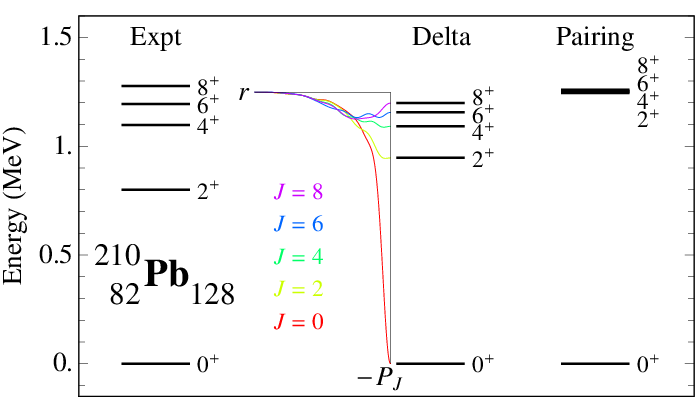
\includegraphics[width=0.6\textwidth]{figure/F_Pb210.png}
\caption{${}^{210}\textrm{Pb}$的低能实验能谱(左),对于一个zero-range delta的对应的能谱(中),以及对应于配对相互作用的能谱(右)。能级由它们的角动量和宇称$J^\pi$标记。插图显示了当两个中子在谐振子的$2g_{9/2}$轨道并且耦合的角动量为$J$时在距离$r$处发现这两个中子的几率密度$P_J$。\label{fig_Pb210}}
\end{figure}

配对相互作用由 Racah 为了原子中电子的分类而引入的。他能导出一个电子间的相互作用能的近似公式,并且可以证明配对相互作用的任意本征态都被一个'seniority 数'$v$表征,其对应于未配对耦合为轨道角动量$L=0$的电子数。Racah 最初对'seniority'的定义是利用分数的系数。后来,他指出可以利用群论来简化。Seniority 变成了在分类中与(酉)辛代数$Sp(2j+1)$相关的一个标记
\begin{equation}\label{eq_dif}
{\setlength\arraycolsep{3pt}\renewcommand{\arraystretch}{1}
\begin{array}{ccccc}
U(2j+1)&\supset&Sp(2j+1)&\supset&SU(2)\\
\downarrow& &\downarrow& &\downarrow\\
\textrm{[}1^{n}\textrm{]}& &[1^\upsilon]& &J
\end{array}}
\end{equation}
因为核子是全同的,$j^n$的配置所有态都属于完全反对称不可约表示$U(2j+1)$的$[1^n]$。因此,$Sp(2j+)$的不可约表示也一定是完全反对称的、属于$[1^\upsilon]$类型的,允许$senirority$的值为$\nu=n,n-2,\cdots,1$或0.

在定义\ref{eq_dif}中,seniority的出现作为与代数$Sp(2j+1)$相关的指标。这样的缺点是,依赖于$j$,代数可能是非常大的。问题可能变得更加复杂,当核子是非全同的,并且具有同位旋$t=\frac{1}{2}$。单粒子态的总数就变成了$\Omega\equiv(2j+1)(2t+1)$,很快就会遇到一个令人生畏的群理论的还原问题。幸运的是,一个更简单的可选择的seniority的定义可以通过代数学的语言给出,其不会随$j$改变。这个想法由Kerman(对于$t=0$的情况(即全同粒子))和Helmers(对于一般的$t$)同时且独立的提出来。其来源于产生和湮灭粒子的的$\hat{S}_+^j$和$\hat{S}_-^j$算符,以及具有第三类产生子$\hat{S}^j_z$(有一个粒子产生同时有一个粒子湮灭的算符)的对易子。这一类算符的集合,即所谓的准自旋算符,在对易下封闭,并且形成(酉)辛代数(Sp(4t+2)),其可以被证明与$Sp(2j+1)$在分类\ref{eq_dif}中引入的的等同的性质。

配对问题的准自旋公式依赖于事实:配对相互作用是与$Sp(4t+2)$代数的二阶 Casimir 算符相关的。这允许对相同粒子$(t=0)$以及中子和质子$(t=\frac{1}{2})$的情况的本征值有个同时且简单的推导。这些年,许多结果都被推导出来了,并且考虑了许多在这两种情况下的扩展,其在下面进行单独的讨论。

\subsubsection{Identical nucleons}

对于$t=0$的情况,其包含了与$\textrm{SU}(2)$同构的代数Sp(2)。由于它与自旋代数有着形式上的相似性,“准自旋”这个名字是由Kerman创造的,而且这个术语适用于所有情况,即使$t\ne0$。准自旋代数Sp(2)\~SU(2)可以被得到,通过注意一点,在二次量子化中,在公式\ref{eq_eq8}中定义的配对相互作用被写为
\begin{equation}\label{eq_Vpair}
\hat{V}_\textrm{pairing}=-g\hat{S}^j_+\hat{S}^j_-
\end{equation}
并且
\begin{equation}
\hat{S}^j_+=\frac{1}{2}\sqrt{2j+1}(a_j^\dag\times a_j^\dag)^{(0)}_0,\quad\hat{S}^j_-=\left(\hat{S}^j_+\right)
\end{equation}
其中$a_{jm_j}^\dagger$在轨道$j$上产生一个投影为$m_j$的核子。不需要同位旋标记$t$和$m_t$来表征同类核子。符号$\times$表示角动量耦合,因此$\hat{S}^j_+$创造了一对角动量耦合为$J=0$的核子。对易子$[\hat{S}^j_+,\hat{S}^j_-]\equiv2\hat{S}^j_z$,和$[\hat{S}^j_z,\hat{S}^j_\pm]=\pm\hat{S}^j_\pm$,表明$\hat{S}^j_+$、$\hat{S}^j_-$和$\hat{S}^j_z$形成了一个封闭的代数SU(2).在SU(2)的基上可以导出几个标志性的结果。准自旋对称性允许配对相互作用的完整本征谱的确定,其由
\begin{equation}
\hat{V}_\textrm{pairing}|j^nvJM_J\rangle=E(n,v)|j^nvJM_J\rangle
\end{equation}
和
\begin{equation}\label{eq_13}
E(n,v)=-\frac{g}{4}(n-v)(2j-n-v+3)
\end{equation}
给出。除了核子数$n$,总角动量$J$以及它的投影$M_J$以外,所有的本征态都通过一个seniority量子数$v$来表征,其表示没有在总角动量耦合为零的配对中的核子数。对于一个相互吸引的配对相互作用($g>0$),其具有最低能量的本征态,如果核子数为偶数时seniority$v=0$,,如果核子数为奇数时seniority$v=1$.这些最低能量的本征态,取决于归一化因子,对于偶数$n$可以被写成$(\hat{S}^j_+)^{n/2}|0\rangle$,对于奇数$n$可以被写成$a_{jm_j}^\dag(\hat{S}^j_+)^{n/2}|0\rangle$,其中$|0\rangle$是核子的真空态。

关于原子核配对关联的讨论,传统上是受到凝聚态超流性处理的启发,其是在1957年由 Bardeen, Cooper 和 Schrieffer 提出,并且后来被用来讨论原子核的配对(Bohr, Mttelson, \&Pines, 1958)。超流相的特征是在单个量子态中存在大量全同的玻色子。在超导体中的玻色子是在费米面处形成的具有相反动量的电子对,而在原子核中,根据前面的讨论,它们是具有相反角动量的价核子对。

这些概念的一般形式涉及到几个轨道。在简并轨道的情况下,这可以通过替换来实现$\hat{S}_\mu^j\mapsto\hat{S}_\mu\equiv\sum_j\hat{S}^j_\mu$,这使得前面的所有结果对单$j$有效,保持不变。后面的公式可以应用于单幻核,但由于它需要配对相互作用与简并轨道的的假设,因此其适用性受到限制。

Richardson 在Bethe假设的基础上,提出了一种求解分布在非简并能级上的粒子间通过对力发生相互作用的问题的精确方法,并将其推广到其他可积配对模型中。Richardson 方法的证明可以通过用非简并单粒子能量补充配对相互作用\ref{eq_Vpair},以获得以下哈密顿量:
\begin{equation}\label{eq_hamilton4}
\hat{H}_\textrm{pairing}=\sum_j\epsilon_j\hat{n}_j-g\hat{S}_+\hat{S}_-
\end{equation}
其中$\hat{n}_j$是轨道$j$的数量算符,$\epsilon_j$是轨道的单粒子能,并且$\hat{S}_\pm=\sum_j\hat{S}^j_\pm$。哈密顿量\ref{eq_hamilton4}的可解性来自于$\textrm{SU}(2)\bigotimes\textrm{SU}(2)\bigotimes\cdots$对称性,其中每一个$\textrm{SU}(2)$代数对应于一个特定的$j$。本征态的形式是
\begin{equation}\label{eq_prod}
\prod_{p=1}^{n/2}\left(\sum_j\frac{\hat{S}_+^j}{2\epsilon_j-E_p}\right)|{\rm o}\rangle
\end{equation}
其中$E_p$是$n/2$耦合的解,非线性Richardson方程
\begin{equation}
\sum_j\frac{\Omega_j}{2\epsilon_j-E_p}-\sum_{p'(\ne p)}^{n/2}\frac{2}{E_{p'}-E_p}=\frac{1}{g},\quad p=1,\ldots,n/2
\end{equation}
其中$\Omega_j=j+1/2$。这个方程可以用图解的方式求解,图\ref{F_richardson}给出了一个简单的$n=2$的情况。在乘积\ref{eq_prod}中的每一对都通过依赖于能量$E_p$系数$\alpha_j=(2\epsilon_j-E_p)^{-1}$来定义,其中$p$标记$n/2$对。Bethe假设的一个特点是它不再由相同对的叠加组成,因为当$p$变换时,系数$(2\epsilon_j-E_p)^{-1}$从1变到$2/n$。因此,Richardson的模型提供了一个解,满足所有可能的从具有超流性质到具有很少或没有对关联性质的哈密顿量\ref{eq_hamilton4}。这个解能否被称为超流的取决于与强度$g$相关的差异$\epsilon_j-\epsilon_{j'}$。
\begin{figure}[H]
\centering
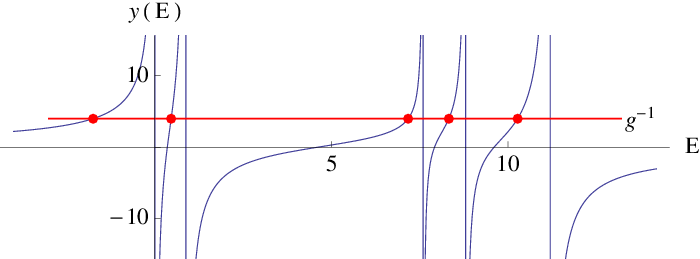
\includegraphics[width=0.6\textwidth]{figure/F_richardson.png}
\caption{两个核子在5个单粒子轨道上的分布的 Richardson 方程的图形解。求和 $\Sigma_j\Omega_j/(2\epsilon_j-E)\equiv y(E)\ (\textrm{in MeV}^{-1})$ 作为 $E$ (in MeV) 的函数被画出。该曲线 (blue) 与曲线 ${y=1/g}$ (red) 的交点 (red dots) 对应于 Richardson 方程的解。\label{F_richardson}}
\end{figure}


配对哈密顿量\ref{eq_hamilton4}允许非简并的单粒子轨道$\epsilon_j$,但是要求强度$g$是独于$j$的常数。或者,一个具有简并单粒子轨道的哈密顿量$\epsilon_j=\epsilon$,但是强度$g_j$是轨道依赖的
\begin{equation}
\hat{H}'_\textrm{pairing}=\epsilon\sum_j\hat{n}_j-\sum_jg_j\hat{S}^j_+\sum_{j'}g_{j'}\hat{S}^{j'}_-
\end{equation}
基于Bethe假设,其也能被精确求解。然而,对于具有任意非简并的单粒子轨道$\epsilon_j$和任意轨道相关强度$g_j$的配对哈密顿量,除了在两轨道的情况下,还没有确切的解。$\epsilon_j=g_j^2$的情况也是可解的,并且被应用在重核中。到目前为止,讨论都仅限于两个轨道$j$和$j'$之间的强度为$g_{jj'}$的可分离的相互作用,其中$g_{jj'}$的可被分解为$g_{jj'}=g_jg_{j'}$。不可分离的配对相互作用的精确解也可以通过结合运动的有理和双曲积分的得到,在综述(Dukelsky, Pittel, \& Sierra, 2004)有讨论这个问题。

尽管存在这些可能的推广,但应该记住,配对相互作用只是核子之间实际的残余相互作用的近似,如图\ref{fig_Pb210}所示。为了得到更加普适的方法,对壳模型的哈密顿量\ref{eq_hamilton3}考虑如下的条件:
\begin{equation}\label{eq_18}
[[\hat{H}_{\rm GS},\hat{S}_+^\alpha],\hat{S}_+^\alpha]=\Delta\left(\hat{S}^\alpha_+\right)^2
\end{equation}
其中$\Delta$是一个常数,$\hat{S}_+^\alpha=\Sigma_j\alpha_j S_+^j$产生$\hat{H}_{\rm GS}$的能量为$E_0$的最低的两粒子本征态,$\hat{H}_{\rm GS}\hat{S}_+^\alpha|{\rm}\rangle=E_0\hat{S}_+^\alpha|{\rm}\rangle$。由Talmi提出的推广了的seniority的条件要比配对相互作用的假设要弱得多,并且它不需要对易子$[\hat{S}_+^\alpha,\hat{S}_-^\alpha]$产生(取决于一个常数)数量算符,这个算符是准自旋公式的核心。尽管没有一个封闭的代数结构,但是仍然有可能计算出满足条件\ref{eq_18}的哈密顿量的精确解。对于偶数个核子,它的基态具有与准自旋形式相同的简单结构
\begin{equation*}
\hat{H}_{\rm GS}\left(\hat{S}_+^\alpha\right)^{n/2}|{\rm o}\rangle=E_{\rm GS}(n)\left(\hat{S}_+^\alpha\right)^{n/2}|{\rm o}\rangle
\end{equation*}
具有对应任意的核子数$n$都可以被计算得到的能量
\begin{equation*}
E_{\rm GS}(n)=nE_0+\frac{1}{2}n(n-1)\Delta
\end{equation*}
由于它是线性和二次依赖于核子数$n$的,所以这个结果可以被认为是一个Racah's seniority公式\ref{eq_13}的推广,当$E_0=-g(j+1)/2$和$\Delta=g/2$时可以化简得到。

\subsubsection{Neutrons and protons}

对于$t=\frac{1}{2}$的情况,可以得到准自旋代数Sp(4),其是与SO(5)同构的。代数Sp(4)与SO(5)由两个指标表征,对应于 seniority $v$和约化同位旋$T_v$。Seniority $v$与在类核子的情况下的解释是相同的,即没有配对耦合成角动量$J=0$的核子数,而约化同位旋对应于这些核子总的同位旋。

前面的结果可以由 Helmers 提出的对任意$t$的一般性分析得到。 有兴趣的话可以明确的分析在原子核中适用的选择,即$t=\frac{1}{2}$。 最后给出了在 $LS$ 耦合中的结果,这是推广到中子和质子的更方便的方案。

如果$\ell$壳层包含质子和中子,那么对相互作用就被假定是同位旋不变的,这表明在$T=1$的三种可能的,即中子-中子、质子-质子、质子-中子的情况下是相同的,并且配对相互作用\ref{eq_Vpair}采用的形式是
\begin{equation}\label{eq_19}
\hat{V}_\textrm{pairing}'=-g\sum_\mu\hat{S}_{+,\mu}^\ell\hat{S}_{-,\mu}^\ell\equiv-g\hat{S}_+^\ell\cdot\hat{S}_-^\ell
\end{equation}
其中点表示在同位旋中的标量积。表示为核子算符$a^\dag_{\ell m_\ell,sm_s,tm_t}$,其现在也带有同位旋指标(当$t=\frac{1}{2}$),配对算符是
\begin{equation}\label{eq_20}
\hat{S}^\ell_{+,\mu}=\sqrt{\frac{1}{2}}\sqrt{2\ell+1}(a^\dag_{\ell,s,t}\times a^\dag_{\ell,s,t})^{(001)}_{00\mu},\quad\hat{S}^\ell_{-,\mu}=\left(\hat{S}^\ell_{+,\mu}\right)
\end{equation}
其中$\hat{S}$表示轨道角动量$L=0$,自旋$S=0$,以及同位旋$T=1$的对。指标$\mu$(同位旋投影)用来区分中子-中子对($\mu=+1$)、质子-质子对($\mu=-1$)和质子-中子对($\mu=0$)。所以$L=0,\ S=0$以及$T=1$存在3种不同的对(在图顶部),并且通过作用同位旋升降算符$\hat{T}_\pm$联系在一起。与哈密顿量\ref{eq_19}对应的准自旋代数是SO(5),并且这使得这个问题可以解析求解。
\begin{figure}[H]
\centering
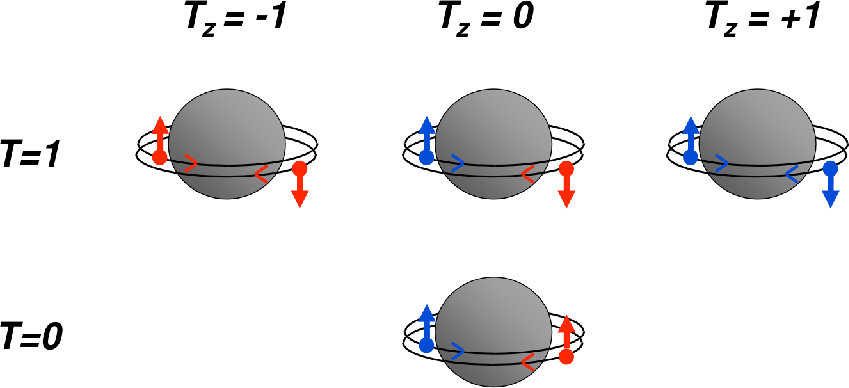
\includegraphics[width=0.6\textwidth]{figure/F_pairs.png}
\caption{轨道角动量$L=0$的不同种类的核子对的示意图。参与配对的价中子(蓝色)或质子(红色)占据时间反转轨道(沿相反方向绕着原子核旋转)。如果核子是相同的,它们的自旋必须是反平行的,这个构型对于中子-质子对也是允许的(顶部)。只有中子-质子对(底部)才允许具有自旋平行的构型。\label{F_pairs}}
\end{figure}

对于一个质子和一个质子,这里存在一个不同的自旋平行的配对状态(图\ref{F_pairs}底部)。因此,对于中子和质子系统最一般的配对相互作用是
\begin{equation}\label{eq_21}
\hat{V}^{''}_\textrm{pairing}=-g\hat{S}^\ell_+\cdot\hat{S}^\ell_--g\hat{P}^\ell_+\cdot\hat{P}^\ell_-
\end{equation}
其中$\hat{P}$表示轨道角动量$L=0$,自旋$S=1$,以及同位旋$T=0$的对
\begin{equation}\label{eq_22}
\hat{P}^\ell_{+,\mu}=\sqrt{\frac{1}{2}}\sqrt{2\ell+1}(a^\dag_{\ell,s,t}\times a^\dag_{\ell,s,t})^{(010)}_{0\mu 0},\quad\hat{P}^\ell_{-,\mu}=\left(\hat{P}^\ell_{+,\mu}\right)
\end{equation}
指表$\mu$是自旋投影,区分$S=1$的对的三个空间方向。配对相互作用\ref{eq_21}现在包含两个参数,$g$和$g'$,分别是同位旋矢量组分和同位旋标量组分的强度。对于不同的比率$g/g'$,得到了在本质上具有不同结构的解。

一般来说,与配对相互作用\ref{eq_21}相关联的问题只能在给定壳模型空间的一个典型的大小的情况下,通过数值方法来解决,这是一项艰巨的任务。然而,对于一些特定的$g$和$g'$,$\hat{V}^{''}_\textrm{pairing}$可以被解析的求解。通过分析发现存在代数SO(8),它是由配对算符\ref{eq_20}和\ref{eq_22},它们的对易子,以及它们自身的对易子,并以此类推直到得到一个封闭的代数结构所构成的的。除了配对算符\ref{eq_20}和\ref{eq_22}以外,还通过数量算符$\hat{n}$,自旋和同位旋算符$\hat{S}$、$\hat{T}$,以及在3.2节Wigner's supermultiplet algebra中义的Gamow-Teller类的算符$\hat{U}_{\mu\nu}$引入了封闭性。

从子代数SO(8)的研究中可以得到在下面的三种情况下:(i)$g=0$, (ii)$g'=0$以及(iii)$g=g'$,配对相互作用\ref{eq_21}具有动力学的对称性,这三种情况分别对应于纯的同位旋标量配对,纯的同位旋矢量配对,以及相等强度的同位旋矢量和同位旋标量配对。在这三个限制下,seniority $v$ 是守恒的,在(i)和(ii)的情形下,seniority $v$ 与SO(5)代数相关,而在(iii)的情形下,seniority $v$ 与so(8)代数相关。

相同核子的配对理论的主要结果之一是从$S$对的角度来认识低能态的特殊结构。因此,在中子与质子的配对理论中解决同样的问题是很有意义的。SO(8)的超流体的性质可以用中子数$N$和质子数$Z$相等的原子核基态的例子来说明。对于相等强度的同位旋矢量和同位旋标量的配对,$g=g'$,配对相互作用\ref{eq_21}是可解的,并且可以证明它的基态是
\begin{equation}\label{eq_23}
\left(\hat{S}_+^\ell\cdot\hat{S}_+^\ell-\hat{P}_+^\ell\cdot\hat{P}_+^\ell\right)^{n/4}|\textrm{o}\rangle
\end{equation}
这表明,超流体的解具有四重结构,即它还原为玻色子类物体的凝聚态,对应于四个核子。以为这个物体在自旋和同位旋中的标量,所以它可以被考虑为一个$\alpha$粒子,然而,它的轨道特性可能与实际的$\alpha$粒子不同。在SO(8)的其他两个限制下,$g=0$和$g'=0$,也表现出了一个四重结构,具有与\ref{eq_23}同一类的基态波函数,只是其中第一项或第二项被抑制。因此,对于具有任意强度$g$和$g'$的配对相互作用\ref{eq_21}的$N=Z$核的基态波函数的一个合理的假设是
\begin{equation}\label{eq_24}
\left(\cos\theta\hat{S}^\ell_+\cdot\hat{S}^\ell_+-\sin\theta\hat{P}_+^\ell\cdot\hat{P}_+^\ell\right)^{n/4}|\textrm{o}\rangle
\end{equation}
其中$\theta$是一个依赖于$g/g'$比率的参数。

类$\alpha$粒子的凝聚态\ref{eq_24}可以被看做是$N=Z$的$g$和$g'$的任意组合的配对相互作用\ref{eq_21}基态的极好的近似。然而,应强调的是,在价核子壳中当中子和质子同时存在时,配对相互作用\ref{eq_21}不是一个包含重要的四极组分的真实壳模型哈密顿量的很好的近似。因此,任何仅基于$L=0$的费米子对的模型,在本质上都必须是示意性的。一个真实的模型也应该包括$L\ne0$的对。

\subsection{Wigner's supermultiplet model}

Wigner 的超多重模型假定核力在自旋和同位旋空间中是转动不变的。具有这样的性质的壳模型的哈密顿量满足下面的对易关系:
\begin{equation}\label{eq_25}
[\hat{H},\hat{S}_\mu]=[\hat{H},\hat{T}_\mu]=[\hat{H},\hat{U}_{\mu\nu}]=0
\end{equation}
其中
\begin{equation}\label{eq_26}
\hat{S}_\mu=\sum_{k=1}^A\hat{s}_{k,\mu},\qquad\hat{T}_\mu=\sum_{k=1}^A\hat{t}_{k,\mu},\qquad\hat{U}_{\mu\nu}=\sum_{k=1}^A\hat{s}_{k,\mu}\hat{t}_{k,\nu}
\end{equation}
是自旋、同位旋和自旋-同位旋算符,而$\hat{s}_{k,\mu}$和$\hat{t}_{k,\mu}$是第$k$个核子的自旋和同位旋组分。15算符\ref{eq_26}产生李代数SU(4)。根据在第2节中的讨论,任意满足条件\ref{eq_25}的哈密顿量都具有SU(4)对称性,除此之外还有与总自旋$S$和总同位旋$T$守恒有关的对称性。

Wigner 的超多重态分类的相关的物理,是因为具有空间对称性的态在能量上是受到青睐的,因此剩余相互作用具有短程吸引的性质所导致的。为了对SU(4)对称性有一个定性的认识,分析两个核子的情况是具有指导意义的。波函数的完全反对称性要求空间部分是对称的,自旋-同位旋部分是反对称的,反之亦然。这两种情况都对应于SU(4)下的不同对称性,第一种是反对称的,第二种是对称的。在给定代数下的对称性可以用所谓的{\emph Young tableau} 来描述。对于两个核子的情况,对称和反对称的不可约表示的标记分别是
\begin{equation*}
\Box\Box\equiv[2,0],\qquad\begin{array}{c}
\Box\\[-2.5ex]
\Box
\end{array}\equiv[1,1]
\end{equation*}
并且 Young tableaux 是共轭的,即,可以交换一个的行和列来得到另一个。这个结果可以推广到多个核子的情况,并且得到一个结论:一个态的能量依赖于它的SU(4)标记,其在这里标记为3个数$(\bar{\lambda},\bar{\mu},\bar{\nu})$。

Wigner 的超多重模型是一种不适合于原子核的$LS-$耦合的方法。尽管 Wigner 的思想适用性有限,但它仍然很重要,因为它证明了剩余相互作用的短程特性与多体波函数的空间对称性之间的联系。SU(4)对称性的破坏是壳模型哈密顿量\ref{eq_hamilton3}中自旋轨-道项的结果,它不满足方程\ref{eq_25}中的第一个和第三个对易关系。自旋-轨道项破坏了SU(4)对称性[SU(4)不可约表示被它混合了],并且在较重的原子核中越来越多地出现这样的情况,因为自旋双重态的能量劈裂随着核子数$A$的增加而增大。

\subsection{Elliott's rotation model}

在 Wigner 的超多重模型中,波函数的空间部分用总轨道角动量$L$来表征,但在其他方面未作说明。Elliott 模型的主要特点是它提供了额外的与形变核相关的附加轨道量子数。转动的 Elliott 模型以 Wigner 的SU(4)分类为前提,此外还假设剩余相互作用具有四极性,如果价壳层中包含中子和质子,那么这是一个合理的假设。其中一个需要把壳模型的哈密顿量\ref{eq_hamilton3}简化为
\begin{equation}\label{eq_27}
\hat{H}_\textrm{SU(3)}=\sum_{k=1}^A\left(\frac{\hat{p}^2_k}{2m_k}+\frac{1}{2}m_k\omega^2r^2_k\right)+\hat{V}_\textrm{quadrupole}
\end{equation}
其中$\hat{V}_\textrm{quadrupole}=-g_2\hat{Q}\cdot\hat{Q}$包含一个四极算符
\begin{equation}\label{eq_28}
\hat{Q}_\mu=\sqrt{\frac{3}{2}}\left[\sum_{k=1}^A\frac{1}{b^2}(\bar{r}_k\wedge\bar{r}_k)_\mu^{(2)}+\frac{b^2}{\hbar^2}\sum_{k=1}^A)(\bar{p}_k\wedge\bar{p}_k)_\mu^{(2)}\right]
\end{equation}
其中$\bar{r}_k$和$\bar{p}_k$是核子$k$的坐标和动量,$b$是核子的长度参数,$b=\sqrt{\hbar/m_n\omega}$,$m_n$是核子的质量。利用在第2节中讨论的技巧,可以证明壳模型哈密顿量\ref{eq_27}是可以解析求解的。因为哈密顿量\ref{eq_27}满足对易关系\ref{eq_25},并且它的本征态由相应于多重标记$(\bar{\lambda},\bar{\mu},\bar{\nu})$的量子数表征。自旋-同位旋的对称性SU(4)轨道对称${\rm U(\Omega)}$共轭等价,${\rm \Omega}$标记轨道壳的大小(例如,对于$s, p, sd,\cdots$壳,${\rm \Omega}=1,3,6,\cdots $)。然而,根据代数的嵌套链${\rm U(\Omega)}\supset SU(3)\supset SO(3)$,${\rm U(\Omega)}$不是哈密顿量\ref{eq_27}的一个真实的对称性,而是一个破缺。由此,我们可以发现哈密顿量\ref{eq_27}具有本征态$|[1^n](\bar{\lambda},\bar{\mu},\bar{\nu})(\lambda,\mu)K_LLM_LSM_STM_T$,其能量为
\begin{equation*}
E_\textrm{SU(3)}(\lambda,\mu,L)=E_0-g_2[4(\lambda^2+\mu^2+\lambda\mu+3\lambda+3\mu)-3L(L+1)]
\end{equation*}
其中$E_0$是与哈密顿量\ref{eq_27}的第一项相关的能量常数。除了在Wigner 的超多重模型中考虑的量子数集合即:SU(4)的标记$(\bar{\lambda},\bar{\mu},\bar{\nu})$、总的轨道角动量$L$和它的投影$M_L$、总自旋$S$和它的投影$M_S$、总的同位旋$T$和它的投影$M_T$外,哈密顿量\ref{eq_27}的所有本征态都由SU(3)的量子数$(\lambda,\mu)$以及额外的标记$K_L$来表征。每一个不可约表示$(\lambda,\mu)$都包含一个典型的在某个上限处被截断的转动带的轨道角动量$L$。标记$K_L$定义了与该带相关联的内禀态,并且可以解释为轨道角动量$L$在转动形变核的对称轴上的投影。

Elliott 的方法的重要性在于它通过混合球形结构产生了态的转动分类。利用SU(3)模型首次揭示了如何通过球壳模型产生形变核的形状的。因此,Elliott 的工作弥补了球形核壳模型和几何集体模型之间的差距,在此之前它们仍是作为核的独立图像而存在。

Elliott 的SU(3)模型对普遍存在于原子核中的转动现象提供了一种自然解释,但是它是通过假设 Wigner 的SU(4)对称性来实现的,而 Wigner 的SU(4)对称性在大多数原子核中都是被严重破坏。自从 Elliott 以来,这个谜团已经激发了很多工作:如何从适用于大多数核的$-$耦合图像开始理解核中的转动现象?多年来已经提出了几个方案,目的是将SU(3)方案转换到那些修正过的情况。Zuker 等人就提出了一个这样的修正,名为准SU(3),并引用了$jj-$和$LS$耦合图像中四极算符的矩阵元的相似性。

可以说,将SU(3)模型应用于重核的最成功方法是基于赝自旋对称的概念。解释这种对称性的出发点是哈密顿量\ref{eq_hamilton3}的单粒子部分。对于$\zeta_{\ell\ell}=\zeta_{\ell s}=0$,我们得到了一个三维各向同性谐振子,它表现出与U(3)对称性相关的简并。对于任意非零的$\zeta_{\ell\ell}$和$\zeta_{\ell s}$,这个对称性是破缺的。然而,对于特定的$4\zeta_{\ell\ell}=\zeta_{\ell s}$的组合,在单粒子谱中恢复了某种程度的简并性(见图\ref{F_qpsu3}),这与所谓的赝自旋对称有关。
\begin{figure}[H]
\centering
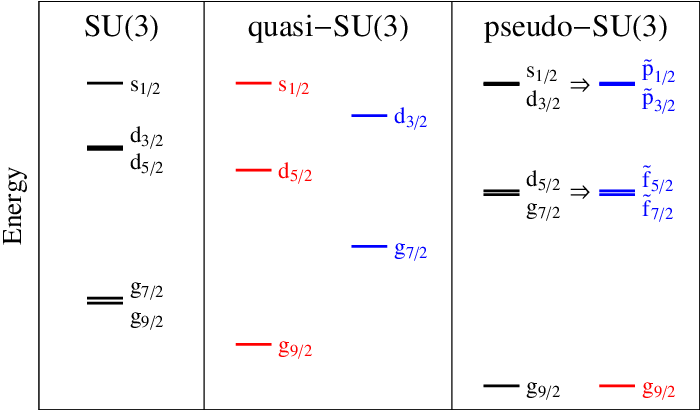
\includegraphics[width=0.6\textwidth]{figure/F_qpsu3.png}
\caption{以 $sdg$ 振动壳为例,在 SU(3)、准 SU(3) 和赝 SU(3) 下,具有非零的二次轨道强度 $\zeta_{\ell\ell}\ne0$ 的单粒子能级。其自旋-轨道强度在SU(3)下 $\zeta_{\ell s}\approx0$ ,在准SU(3)下 $\zeta_{\ell s}\approx2\zeta_{\ell\ell}$ ,在赝SU(3)下 $\zeta_{\ell s}\approx4\zeta_{\ell\ell}$。红色和蓝色的单粒子空间被假定为近似解耦的。在赝 SU(3) 中,能级简并可以用赝自旋对称性来解释。\label{F_qpsu3}}
\end{figure}

赝自旋对称在核物理中有着悠久的历史。近四十年前,在核平均场势中几乎存在退化的伪自旋双峰,他指出,由于小的赝自旋-轨道分裂,赝$LS$耦合的合理起点应该是在$LS$耦合变得不可接受的中、重核区域。以赝$LS$耦合为前提,赝SU(3)模型的构造方法与 Elliott 的SU(3)模型在$LS$耦合中的定义方法基本相同。在提出这个建议的许多年以后,Ginocchio 才证明了赝自旋是当标量势和矢量势的大小相等符号相反时的 Dirac 方程的一种对称性。

到目前为止讨论的模型都具有局限于单个壳的性质,无论是谐振子还是赝谐振子壳。对核集体运动的完整描述需要涉及单个(赝)谐振子壳外的结构的关联。这种关联的适当框架引用了非紧代数的概念,与紧代数相比,非紧代数可以具有无穷维酉不可约表示。后一个条件是必要的,因为到高层壳的激发可以是无穷大的。通过在(非紧)辛代数SP(3,R)中嵌入SU(3)代数,Rosensteel和Rowe得到了谐振子的到高壳层的激发。

\subsection{The Lipkin model}

核物理中另一个值得注意的代数模型是Lipkin等人提出的,他考虑了两个能级(由指数$\sigma=\pm$标记),每个简并度为$\Omega$的能级上分布着$n$个费米子。Lipkin 模型具有一个SU(2)代数结构,它的产生是由算符
\begin{equation*}
\hat{K}_+=\sum_ma_{m+}^\dag a_{m-},\quad\hat{K}_-=\left(\hat{K}_+\right)^\dag,\quad\hat{K}_z=\frac{1}{2}(\hat{n}_+-\hat{n}_-)
\end{equation*}
是通过产生和湮灭算符$a_{m+}^\dag$和$a_{m-}$写出来的,其中$m=1,\ldots,\Omega$,$\sigma=\pm$,其中$\hat{n}_\pm$计算在$\sigma=\pm$的能级上的核子数。哈密顿量是
\begin{equation*}
\hat{H}=\epsilon\hat{K}_z+\frac{1}{2}v\left(\hat{K}_+\hat{K}_-+\hat{K}_-\hat{K}_+\right)+\frac{1}{2}\omega\left(\hat{K}_+^2+\hat{K}_-^2\right)
\end{equation*}
利用潜在的SU(2)代数,这个哈密顿量在参数$\epsilon,v,\omega$取确定的值的情况下是可以解析求解的。它们有一个简单的物理意义:$\epsilon$是从更低的$\sigma=-$的能级激发一个核子到$\sigma=-$的更高的能级所需要的能量,$v$ 是混合具有相同核子数$n_-$和$n_+$的构型的相互作用强度,而$\omega$是混合这些数量相差2的不同的构型相互作用的强度。因此,Lipkin 模型具有三种(尽管是示意性的)对确定原子核的结构很重要的成分:价壳层中核子间的相互作用$v$,通过能量$\epsilon$将核子从价壳层激发成更高壳层的几率,将这些粒子-空穴激发与价态混合的相互作用$\omega$。利用这些成分,Lipkin 模型在核物理中提出的各种近似的试验场中起到了重要的作用,其中的例子在参考文献中给出。

\section{Geometric collective models}

在1879年,在研究不可压缩液滴的性质时,Lord Rayleigh发现振动的一般模式可以用出现在液滴半径的展开式中的变量$\alpha_{\lambda\mu}$描述
\begin{equation}\label{eq_29}
R(\theta,\phi)=R_0\left(1+\sum_{\lambda\mu}\alpha_{\lambda\mu}^\ast Y_{\lambda\mu}(\theta,\phi)\right)
\end{equation}
其中$Y_{\lambda\mu}(\theta,\phi)$是球谐函数,$\theta,\phi$是球面角。由于从早期起原子核就被模型化为一个稠密的带电液滴,就像在几何集体模型中已经完成的经典的文章一样,核物理学家很自然地采用了相同的多极参数化\ref{eq_29}。

Lord Rayleigh也指出,与本征频率最低的正常模式相对应的多极性是$\lambda=2$的四极性。四极集体坐标$\alpha_{2\mu}$可以通过$a_{2\mu}=\Sigma_\nu\mathcal{D}_{\nu\mu}^2(\theta_i)\alpha_{2\nu}$转换为内禀轴系,其中$\mathcal{D}_{\nu\mu}^2(\theta_i)$是 wigner $\mathcal{D}$函数,$\theta_i$是把实验室系转动到内禀系得欧拉角。如果内禀坐标系与四极形变椭球的主轴重合,那么$a_{2\mu}$就满足$a_{2-1}=a_{2+1}=0$和$=a_{2-2}=a_{2+2}$,而剩下的两个变量就可以进一步转换成两个坐标$\beta$和$\gamma$,根据$a_0=\beta\cos\gamma$和$a_{2-2}=a_{2+2}=\beta\sin\gamma/\sqrt{2}$。坐标$\beta\ge0$表示球偏差度,而$\gamma$是一个极坐标,限制在$[0,\pi/3]$的范围内。对于$\gamma=0$,对应的内禀形状是轴对称的长椭,而对于$\gamma=\pi/3$,对应的是轴对称的扁椭,$\gamma$的中间值描述的是三轴形状。

液滴的四极振动的经典的问题被 Bohr 量子化了,得到的哈密顿量
\begin{equation*}
\hat{H}_\textrm{B}=\hat{T}_\beta+\hat{T}_\gamma+\hat{T}_\textrm{rot}+V(\beta,\gamma)
\end{equation*}
其中$\hat{T}(V)$表示动能(势能)。动能有三个贡献,保持轴对称性的$\beta$振动,不保持轴对称性的$\gamma$振动,和四极形变物体的转动。 Bohr的分析得到了一个集体的Schr\"{o}dinger方程$\hat{H}_\textrm{B}\Psi(\beta,\gamma,\theta_i)=E\Psi(\beta,\gamma,\theta_i)$,其中
\begin{equation}\label{eq_30}
\hat{H}_\textrm{B}=-\frac{\hbar^2}{2B_2}\left[\frac{1}{\beta_4}\frac{\partial}{\partial\beta}\beta^4\frac{\partial}{\partial\beta}+\frac{1}{\beta^2\sin3\gamma}\frac{\partial}{\partial\gamma}\sin3\gamma\frac{\partial}{\partial\gamma}\right]+\frac{\hbar^2}{8B_2}\sum_{k=1}^3\frac{\hat{L}^{\prime2}_k}{\beta^2\sin^2(\gamma-2\pi k/3)}
\end{equation}
其中$B_2=\rho R_0^5/2$是物质密度为常数的不可压缩核的质量参数。算符$\hat{L}^{\prime}_k$是内禀参考系中角动量的组成部分,其中质数用于区分这些与实验室参考系中角动量的组成部分。特别是,由于转动惯量的$\gamma$依赖性,$\gamma$激发与集体转动强烈耦合。结果表明,$\gamma$激发的耦合不太强,对势能的明智选择很可能会让$\beta$与$\gamma$和$\theta_i$坐标分离。

\subsection{Exactly solvable collective models}

Wilets 和 Jean 提出了一种将 Bohr Hamiltonian\ref{eq_30}解耦为独立微分方程的方法,需要势能的形式是
\begin{equation}
V(\beta,\gamma)=V_1(\beta)+\frac{V_2(\gamma)}{\beta^2}
\end{equation}
得到的耦合的方程是
\begin{equation}\label{eq_32}
\begin{array}{l}
\left[-\frac{1}{\beta^4}\frac{\partial}{\partial\beta}\beta^4\frac{\partial}{\partial\beta}+u_1(\beta)-\varepsilon+\frac{\omega}{\beta^2}\right]\xi(\beta)=0\\[1.5ex]
\left[-\frac{1}{\sin3\gamma}\frac{\partial}{\partial\gamma}\sin3\gamma\frac{\partial}{\partial\gamma}+\sum_{k=1}^3\frac{\hat{L}^{\prime2}_k}{4\sin^2(\gamma-2\pi k/3)}+u_2(\gamma)-\omega\right]\psi(\gamma,\theta_i)=0
\end{array}
\end{equation}
其中$\omega$是分离常数,$\varepsilon=(2B_2/\hbar^2)E$,而$u_i=(2B_2/\hbar^2)V_i(i=1,2)$。只有当常数$\omega$是由第二个方程的解得到的时候,第一个方程才能够被精确求解。到目前为止,唯一已知的 Bohr 哈密顿量\ref{eq_32}的解析解是当势能是独立于$\gamma$的,即$V_2(\gamma)=0$。在这种情况下,仍然需要决定在方程\ref{eq_32}中的$\omega$的允许的取值。人们提出了许多依靠代数或解析方法求解这一方程的技巧。Rakavy注意到方程\ref{eq_32}的前两项对应于在五维情况下的正交群 SO(5) 中的 Casimir 算符,因此,由群论的讨论可知$\omega$的取值需要满足$\omega=v(v+3), v=1,2,\ldots$,得到如下关于$\beta$的方程
\begin{equation}\label{eq_33}
\left[-\frac{1}{\beta^4}\frac{\partial}{\partial\beta}\beta^4\frac{\partial}{\partial\beta}+u_1(\beta)-\varepsilon+\frac{v(v+3)}{\beta^2}\right]\xi(\beta)=0
\end{equation}
对$u_1(\beta)$[或$V)_1(\beta)$]的特殊选择就可以得到如下的玻尔哈密顿量\ref{eq_30}的精确解。
\vskip 0.6cm
\noindent\textbf{\large The five-dimensional harmonic oscillator.}
\vskip 0.3cm
四极谐振子势是第一个用在一个精确可解的集体模型中的势。势函数$V(\beta,\gamma)$约化为一项$V(\beta)=C_2\beta^2/2$,其中$C_2$是一个常数。尽管人们并不期望在原子核的实验研究中出现四极谐波振动,但该模型还是一个有趣的基准。由关于$\beta$的微分方程的解得到的能谱是$E(n,v)=\hbar\Omega(2n+v+5/2)$其中$\Omega=\sqrt{C_2/B_2}$已经相应的本征波函数是$v+3/2$阶的相关勒让德多项式。能量谱的特征是随着$n$和$v$的增加而增加的简并。谐振子势的 Bohr 哈密顿量的的完整的解可以由基于约化$\textrm{U(5)}\supset\textrm{SO(5)}\supset\textrm{SO(3)}$的群论方法得到。另一种推导是基于前面讨论的准自旋的概念,对于玻色子,准自旋的代数结构是SU(1,1)。
\vskip 0.6cm
\noindent\textbf{\large The infinite square-well potential.}
\vskip 0.3cm
Wilets 和 Jean 证明了五维谐振子势的能谱可以通过引入一个具有无限深方阱形式的$\beta$势来实现非谐,即当$\beta\le b$时$V(\beta)=\textrm{constant}$,当$\beta>b$时$V(\beta)=\infty$。这得到的方程\ref{eq_33}的解是贝塞尔函数,通过在$\beta=b$处波函数消失的边界条件可以得到$v$的允许值。

这个问题的解在很久以后才由 Iachello 在研究从球形到$\gamma$软的势的形状跃迁的时候得到。能谱由能量的本征值决定
\begin{equation*}
E(i,v)=\frac{\hbar^2}{2B_2}k^2_{i,v},\quad k_{i,v}=\frac{x_{i,v}}{b}
\end{equation*}
以及相应的本征波函数
\begin{equation*}
\xi_{i,v}(\beta)\propto\beta^{-3/2}J_{v+3/2}(k_{i,v}\beta)
\end{equation*}
其中$x_{i,v}$贝塞尔函数$J_{v+3/2}$的第$i$个零。因此,如参考文献中详细讨论的,这个解称为E(5)被证明是精确的。
\vskip 0.6cm
\noindent\textbf{\large The Davidson potential.}
\vskip 0.3cm
类似于由Davidson提出的用于分子物理学的三维势的五维势,产生了 Bohr 哈密顿量的另一个解析解。保留了$\gamma$独立性的约束,将前面的谐波势修改为$V(\beta)=C_2(\beta^2+\beta_0^4/\beta^2)/2$。附加项将球形势变为形变势,其最小值位于$\beta_0$。可以由球形势的能谱做替换$v\mapsto\tilde{v}$,其中$\tilde{v}$的定义来自于$\tilde{v}(\tilde{v}+3)=v(v+3)+k\beta_0^4$,而$k=B_2C_2/\hbar^2$,得到修正后的能谱。图\ref{F_davidson}展示了得到的能谱。还研究了质量参数$B_2$依赖于坐标$\beta$的相应的问题。如果考虑$B_2=B_2(0)/(1+a\beta^2)^2$,这个问题就变成了可精确求解的了,利用来自超对称量子力学的技巧,以及通过施加可积条件,也被称为形状不变性。
\begin{figure}[H]
\centering
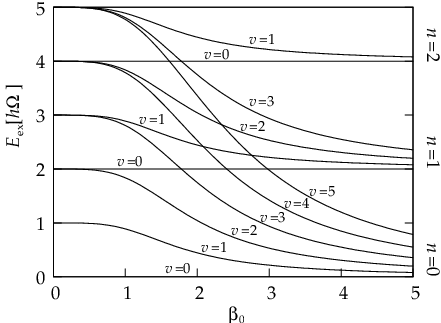
\includegraphics[width=0.6\textwidth]{figure/F_davidson.png}
\caption{Davidson 势能的能谱$E(n,\bar{v})=2n+\bar{v}+5/2$(单位为$\hbar{\rm \Omega}$),作为形变参数$\beta_0$的函数。\label{F_davidson}}
\end{figure}
\vskip 0.6cm
\noindent\textbf{\large Other analytic solutions.}
\vskip 0.3cm
其他使得方程\ref{eq_33}可解的$\gamma$独立的势$V(\beta)$,也可以得到可精确求解的 Bohr 哈密顿量。最值得注意的是,它们是库伦势$V(\beta)=-A/\beta$以及 Kratzer 势$V(\beta)=-B[\beta_0/\beta-\beta_0^2/(2\beta^2)]$。形如$V(\beta)=\beta^{2n},\ (n=1,2,\ldots)$的势也被研究了,对于$n=1$其可以被约化为5维谐振子,而对于$n=\infty$,其可以用数值方法逼近无线深方势阱的情况。L\'{e}vai和Arias 提出了一六次多项式势,得到了一个准可精确求解的模型,它可以简化为一类包含$\beta^2$、$\beta^4$、$\beta^6$项的两参数势。这个选择得到了在态的有限子集中由精确解的 Bohr 哈密顿量,这里特指最低的几个本征态(能量,波函数以及$B(E_2)$值的一个子集)。最后,由 Ginocchio 提出的,特别选择的$V(\beta)=C_2b\beta^2/(1+b\beta^2)$也是可解的。它得到的 Bohr 哈密顿量的解重现了一个非谐振子[或是 IBM 的U(5)极限,见下文]的最低能量本征值。

\subsection{Triaxial models}

许多核可能表现出对轴对称的偏移,需要在 Bohr 哈密顿量中引入明确的三轴特征。由于 Bohr 哈密顿量中振动自由度和转动自由度的耦合,具有$\gamma$依赖性的势即使是可分离的,$V(\beta,\gamma)=V_1(\beta)+V_2(\gamma)$,也允许很少的精确解。早期为了将其应用于更复杂的情况,在绝热近似下对三轴转子进行了研究,即原子核的内禀形状在转动的影响下不会改变。这样的系统,在 Bohr 哈密顿量的背景下,对应于势能的形式是$V(\beta,\gamma)=\delta(\beta-\beta_0)\delta(\gamma-\gamma_0)$,并且它们的哈密顿量只包含转动动能项。另一方面,在 Bohr 哈密顿量出现之前,Reiche 和 Casimir 从旋转物体的经典描述开始,已经对刚性转子的转动的量子力学有了很多研究。两种方法产生的惯性矩不同,在下面进行了讨论。
\vskip 0.6cm
\noindent\textbf{\large Rigid rotor models.}
\vskip 0.3cm
Davdov 及其合作者在 Bohr 哈密顿量的背景下研究并求解了一个三轴转子模型,在绝热近似下,其转动部分简化为
\begin{equation}\label{eq_34}
\hat{H}_\textrm{rot}=\frac{\hbar^2}{8B_2}\sum_{k=1}^3\frac{\hat{L}^{\prime2}_k}{\beta_0^2\sin^2(\gamma_0-2\pi k/3)}
\end{equation}
其中$\beta_0$和$\gamma_0$是固定值,定义转动核的形状。转动惯量${\cal J}_k=4B_2\beta_0^2\sin^2(\gamma_0-2\pi k/3)$对形状参数$\beta_0$和$\gamma_0$的依赖是类似于一个无旋流的液滴的依赖性的,即它的速度场$\bar{v}(\bar{r})$满足条件$\bar{\nabla}\wedge\bar{v}(\bar{r})=0$。

Davydov模型是可精确求解的,因为最低自旋态$L^\pi=0^+,2^+,3^+,\dots$的能量可以用封闭的形式导出。对于更高的自旋态,能量是作为更高阶代数方程的解来获得的:三阶可以得到$L^\pi=4^+$对应的能量,四阶可以得到$L^\pi=6^+$对应的能量,等等。对应的波函数只依赖于欧拉角$\theta_i$,可以写为$\Phi_{iLM}(\theta_i)=\sum_Ka_K^i\Phi_{KLM}(\theta_i)$,其中系数$a_K^i$可由相同的代数方程得到,并且
\begin{equation*}
\Phi_{KLM}(\theta_i)=\sqrt{\frac{2L+1}{16\pi^2(1+\delta_{K0})}}\left[{\cal D}_{MK}^L(\theta_i)+(-)^L{\cal D}_{M,-K}^L(\theta_i)\right]
\end{equation*}
其中${\cal D}^L_{MK}(\theta_i)$是$ Wigner {\cal D}$函数。这些表达式也可以计算电磁跃迁。

另一方面,四极形变刚体的转动惯量的经典表达式是${\cal J}_k=(2m_{\rm n}AR_0^2/5)[1-\sqrt{5/4\pi}\beta_0\cos(\gamma_0-2\pi k/3)]$,其中$m_{\rm n}A$是质量。结果,它的量子力学转动得到了一个不同于玻尔哈密顿量的能谱(见图\ref{F_davydov})。当 Davydov 模型中的一个惯性矩发散时,两种情况之间的最明显区别发生在轴对称极限处($\gamma_0=0$或$\gamma_0=\pi/3$)。这种发散性是由于刚性转动的极值图引起的,当刚性三轴转子模型是由在$\beta$和$\gamma$自由度中允许软化的情况下得到的,这种情况就消失了。
\begin{figure}[H]
\centering
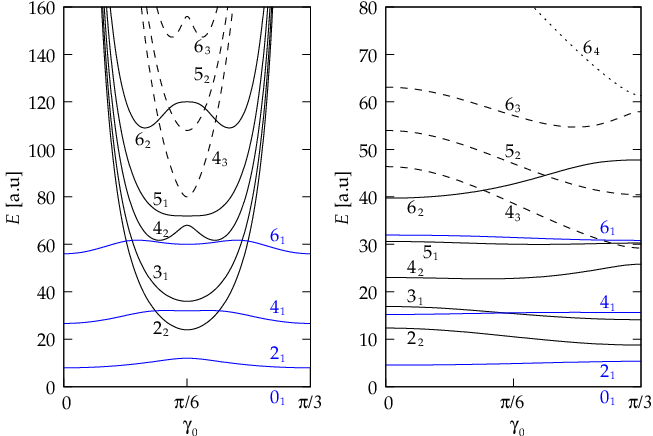
\includegraphics[width=0.6\textwidth]{figure/F_davydov.png}
\caption{刚性转子的能谱,非旋的(左边)和刚性的(右边)转动惯量的值\label{F_davydov}},能量的单位分别是$\hbar^2/(8B_2)$和$5\hbar^2/(4m_{\rm n}AR_0^2$。两种情况下都是$\beta_0=1$。
\end{figure}
\vskip 0.6cm
\noindent\textbf{\large The Meyer-ter-Vehn model.}
\vskip 0.3cm
Meyer-ter-Vehn 发现了一个$\gamma_0=\pi/6$的刚性转子的一个有趣的解。对于这个$\gamma_0$的值,虽然三个内禀的四极矩都是不同的,但是\ref{eq_34}式中的转动惯量${\cal J}_2$和${\cal J}_3$却是相等的。哈密顿量\ref{eq_34}可以重写为$\hbar^2/(2B_2\beta_0^2)(\hat{L}^{\prime2}-3\hat{L}^{\prime2}/4)$,能量本征值为$\hbar^2/(2B_2\beta_0^2)[L(L+1)-3R^2/4]$,其中$L$表示角动量,$R$表示$L$在1-轴(垂直于3-轴)上的投影,对于这样的系统,$R$是一个好量子数。该模型可通过将奇数粒子耦合到三轴转子上用于奇质量核。
\vskip 0.6cm
\noindent\textbf{\large Approximate solutions for soft potentials.}
\vskip 0.3cm
虽然刚性转子可以作为描述某些原子核的良好起点,但$\gamma$激发和集体转动之间的强耦合需要简单、更真实的模型,特别是对于稀土和锕系元素区域中的强变形原子核。一种方法是假设$\gamma$和$\beta$变量中的谐振子(或其他图像)势,从而可以近似地求解 Bohr 哈密顿量。即便是用允许$\beta$自由度的精确耦合的 Wilets–Jean 类的势,波函数的$(\gamma,\theta_i)$部分的解析解除了假设在$\gamma_0$周围的简谐运动外,还需要转动惯量冻结在某个$\gamma_0$值[与最小的$V(\gamma)势相对应$]。有了这些限制,就可以得到解析解。Bonatsos 等人研究了大量这样的势,导出了Bohr 哈密顿量的特解,其由$V_1(\beta)$和$V_2(\gamma)$的各种表达式表征。这些近似的有效性必须进行数值研究。两个特殊的近似解析解,被广泛地用在稀土区域的实验数据中,被称为X(5)和Y(5)。对应势在$\beta$和$\gamma$中是可分离的,在$\beta$方向使用方阱势,在$\gamma$方向使用$\propto\gamma^2$的谐振子[对于X(5)的解],以及在$\beta$方向使用$\propto(\beta-\beta_0)^2$的谐振子,在$\gamma$方向使用在$\gamma=0$附近的无限深方势阱[对于Y(5)的解]。

在参考文献中还讨论了在$\beta$自由度和$\gamma$自由度两个自由度下表现出软的许多其他的模型。
\vskip 0.6cm
\noindent\textbf{\large Partial solutions.}
\vskip 0.3cm
有一些模型在有限数量的态上是可精确求解的。一个例子是 P\"{o}schl–Teller 势,$V(\gamma)=a/\sin^23\gamma$,其在$J=0$和$J=3$的态上有一个精确解。

\subsection{Geometric collective models: an algebraic approach}

精确可解模型仅适用于特定势场$V(\beta,\gamma)$,且范围明显受限。为了处理一般势$V(\beta,\gamma)$,与玻尔哈密顿量\ref{eq_30}相关的微分方程必须用数值方法求解.在文献中提出了一种基于${\rm SU}(1,1)\otimes{\rm SO}(5)$的代数方法。为了改善五维振子基的收敛性,本文将$\beta$中的SU(1,1)波函数与zai$\gamma$和$\theta_i$中${\rm SO}(5)\supset{\rm SO}(3)$产生的球谐函数直接乘积。这种代数结构允许以封闭解析形式计算势能项和动能项的矩阵元素的一般集合。因此,可以容易地导出谐振子、$\gamma$独立的转子和轴向形变转子的精确解。作为这种方法的一个很好的例子,Davidson 的解可以用闭合形式得到。这种方法(也称为代数集体模型)的优点是,人们可以超越$\beta$和$\gamma$振动模式的绝热分离,通常被看作简谐振动,并测试这种限制。目前,考虑了更现实的势能和动能项,使得数值研究远远超出了本文所考虑的精确可解模型的限制。

\section{The interacting boson model}

在几何集合模型中,找到了 Bohr 哈密顿量中特定势的精确解。它们对应于标准数学函数形式的耦合微分方程的解,与第二节量子$n-$体问题的代数公式没有明显的联系。另外,集体核激发也可以用相互作用玻色子模型(IBM)来描述,而不同的是,相互作用玻色子模型可以用代数语言来描述。

初始版本的 IBM 模型用于处理偶偶核,通过$\ell=0$和$\ell=2$的$s$和$d$玻色子间的相互作用来描述核的性质,并且真空态$|{\rm o}\rangle$表示一个双幻核芯。六个态$s^\dagger|{\rm o}\rangle$和$d^\dagger_m|{\rm o}\rangle,m=0,\pm1,\pm2$之间的酉变换也整体的由$b^\dag_{\ell m}$标记,产生李代数U(6)。

在具有许多价态中子和质子的原子核中,壳模型空间的尺寸大得令人望而却步。如果考虑仅由与角动量$J=0$和$J=2$耦合的核子对构成的壳模型态,则该维数将大大减小。此外,如果从核子对到真正的$s$玻色子和$d$玻色子进行映射,则在壳模型和IBM之间建立了联系。

在玻色子的微观解释中,一个具有$2N_b$个价核子的偶数原子核的低能集体态可以近似为$N_b$个玻色子态。尽管分离的玻色子数$n_s$和$n_d$不一定是守恒的,但它们的和$n_s+n_d=N_b$是守恒的。这意味着玻色子总数守恒的哈密顿量的形式是$\hat H_{\rm IBM}=E_0+\hat H_1+\hat H_2+\hat H_3+\cdots$,其中指标表示在U(6)生成元中相互作用的阶,并且其中的第一项是一个常数,表示核芯的结合能。

最一般的 IBM 哈密顿量的特征,包括至多是两体的相互作用和它的群论性质已经被很好地理解了。在得到其本征解的过程中使用了数值方法,但是,就像在核的壳模型中一样,对于特定选择的玻色子能量和玻色子-玻色子相互作用,量子力学多体问题可以被解析地求解。对于至多具有两个玻色子之间的两体相互作用的IBM哈密顿量,存在有三种不同的解析解或极限:振动的U(5),转动的SU(3)以及$\gamma$-不稳定的SO(6)极限。它们与以下代数格点相关:
\begin{equation}\label{eq_35}
{\rm U(6)}\supset\left\{\begin{array}{c}
{\rm U(5)}\supset{\rm SO(5)}\\
{\rm SU(3)}\\
{\rm SO(6)}\supset{\rm SO(5)}
\end{array}\right\}\supset{\rm SO(3)}
\end{equation}
出现在格点\ref{eq_35}中的代数是由$b_{\ell m}^\dagger b_{\ell^\prime m^\prime}$类算符产生的U(6)的子代数。如果选择能量和相互作用使得$\hat{H}_\textrm{IBM}$约化为属于在格点(35)中嵌套代数链的子代数的 Casimir 算子之和,则根据前面的讨论,本征值问题就可以解析求解,并且与不同 Casimir 算符相关的量子数是守恒的。

IBM的一个重要方面是它的几何解释可以通过相干(或内禀)态获得。IBM 使用的是
\begin{equation*}
|N;\alpha_{2\mu}\rangle\propto
\left(s^\dagger+\sum_\mu\alpha_{2\mu}d^\dagger_\mu\right)^N|{\rm o}\rangle
\end{equation*}
其中$\alpha_{2\mu}$与几何集合模型中的形状变量相似。与那个模型中的方法一样,$\alpha_{2\mu}$可以与 Euler 角$\theta_i$和两个固有形状变量$\beta$和$\gamma$联系起来,这两个变量参数化了在核表面围绕平衡形状附近的四极振动。相干态算符的期望值得到$N,\beta$和$\gamma$的函数表达式。因此,最一般的IBM哈密顿量可以在总量面$E(\beta,\gamma)$中转换。对这一类型的分析表明,IBM的三个极限有简单的几何对应关系,在核中经常遇到。

\subsection{Neutrons and protons: $F$ spin}

认识到$s$玻色子和$d$玻色子可以用耦合到角动量$J=0$或$J=2$的价核子对来标记,这清楚地表明玻色子和壳层模型之间的联系需要区分中子和质子。因此,Arima等人提出的模型的扩展版本与模型的原始版本\textbf{IBM-1}不同,在这个模型中,这个区别被称为\textbf{IBM-2}。

在\textbf{IBM-2}中,总的玻色子数$N_b$是中子和质子玻色子数$N_\nu$和$N_\pi$的和,它们是各自守恒的。\textbf{IBM-2}的代数结构是$U(6)$代数的乘积,${\rm U_\nu(6)\otimes U_\pi(6)}$,由中子的玻色子的算符$b^\dagger_{\nu,\ell m}b_{\nu,\ell'm'}$和质子的玻色子算符$b^\dagger_{\pi,\ell m}b_{\pi,\ell'm'}$组成。\textbf{IBM-2}的模型空间是对称不可约表示乘积,${\rm U}_\nu(6)\otimes{\rm U}_\pi(6)$的$[N_\nu]\times[N_\pi]$。在这个模型空间中,$(N_\nu,N_\pi)$-守恒,最一般的旋转不变的\textbf{IBM-2}哈密顿量是对角化的。

IBM-2 提出了中等质量和重核低能集体性质的唯象描述。特别的是,能谱和${\rm E_2}$和${\rm M1}$跃迁的性质可以用作为价中子和价质子数的函数的全局化参数来再现,但具体核性质的详细描述仍然是一个挑战。IBM-2 的对称性限制的分类和分析比在IBM-1中的相应问题要复杂得多,但是最重要的限制是已知的,其与原子核分析有关。

两种玻色子的存在为对它们分配了$F-$自旋量子数提供了可能性,$F=\frac{1}{2}$,玻色子处于两个可能的电荷态,中子的$M_F=-\frac{1}{2}$和质子的$M_F=\frac{1}{2}$。形式上,$F-$自旋由代数的约化来定义
\begin{equation*}
{\setlength\arraycolsep{3pt}\renewcommand{\arraystretch}{1}
\begin{array}{ccccccc}
{\rm U(12)}&\supset&{\rm U(6)}&\otimes&\big({\rm U(2)}&\supset&{\rm SU(2)}\big)\\
\downarrow& &\downarrow& &\downarrow& &\downarrow\\
\textrm{[}N_b\textrm{]}& &[N_b-f,f]& &[N_b-f,f]& &F
\end{array}}
\end{equation*}
其中$2F$是表征U(6)或U(2)的标签之间的差异,$F=[(N_{\rm b}-f)-f]/2=(N_{\rm b}-2f)/2$。代数U(12)由生成元$b^\dagger_{\rho,\ell m}b_{\rho',\ell'm'}$组成,其中$\rho,\rho'=\nu$或$\pi$,其也包括把一个中子玻色子变成质子玻色子的算符,或反之亦然$(\rho\ne\rho^\prime)$。在这个U(12)代数下,玻色子的对称性表现为对称的不可约表示$[N_、\textrm{b}]$。相反,U(6)和U(2)的不可约表示不必是对称的,但是为了保持U(12)的整体对称性,它们应该是相同的。

$F-$自旋的数学结构与同位旋$T$完全相似。定义了一个$F-$自旋SU(2)代数,它由对角算符$\hat{F}_z=(-\hat{N}_\nu+\hat{N}_\pi)/2$和将中子转换成质子玻色子的升降算符$\hat{F}_\pm$组成。这些是与同位旋产生子$\hat{T}_z$和$\hat{T}_\pm$直接相似的。然而,$F-$自旋和同位旋的物理意义是不同的,因为在IBM-2中,具有同位旋对称性的壳模型哈密顿量的映射不一定产生$F-$自旋守恒的哈密顿量。相反,一个$F-$自旋守恒的IBM-2哈密顿量可能具有或不具有好的同位旋的本征态。如果中子和质子占据不同的壳层,从而玻色子被定义在不同的壳层中,那么任何IBM-2哈密顿量都具有对应于具有好的同位旋的壳模型态的本征态,而不管其$F-$自旋对称性如何。另一方面,如果中子和质子占据同一个壳层,一般的IBM-2哈密顿量不会导致具有好的同位旋的态。同位旋对称性破坏在中子和质子近似相等$(N\sim Z)$的原子核中特别显著,需要考虑IBM-3。随着同一壳层中中子和质子数目的不同的增加,$F-$自旋和同位旋的近似等价性得到恢复,对IBM-3的需要消失。

正如核的同量异位的多重态是通过升降算符$\hat{T}_\pm$所隐含的联系来定义的一样,$F-$自旋多重态也可以通过$\hat{F}_\pm$的作用来定义。这些连接的态是在$N_\nu+N_\pi$为常数的核中的;这些核可以是同量异位的(核质量数$A$为常数),也可以是$\alpha$粒子的倍数,这取决于中子玻色子和质子玻色子是相同类型的还是不同类型的(这里是指它们的粒子性或空穴性)。

F自旋多重态的现象学与同量异位素的多重态的现象学相似,但有一个重要的区别。核子-核子相互作用有利于空间对称构型,因此低能下的核激发通常具有$T=T_{\rm min}=|(N-Z)/2|$。玻色子-玻色子相互作用也有利于空间对称性,但这会导致$F=F_{\rm max}=(N_\nu+N_\pi)/2$的低能级。结果,在$F-$自旋多重态的情况下,多重态中的原子核的低能谱之间隐含着一种关系,而同量异位素的多重态(满足$T\ge1$)涉及某些原子核中处于较高激发能的态。

IBM-2的另一个重要方面是,它预测的在IBM-1中发现的态之外的态。它们的结构可以按照如下的理解。具有最大$F-$自旋$F=N/2$的态,,具有U(6)对称性,并且与IBM-1的态是完全类似的。下一类态的$F=N/2-1$在U(6)中不再是对称的,而是属于它的不可约表示$[N-1,1]$。1984年,Iachallo从理论上研究了这种状态,并在${}^{156}$Gd首次观测到,后来在许多其他变形核和球形核中也观测到了。
\begin{figure}[H]
\centering
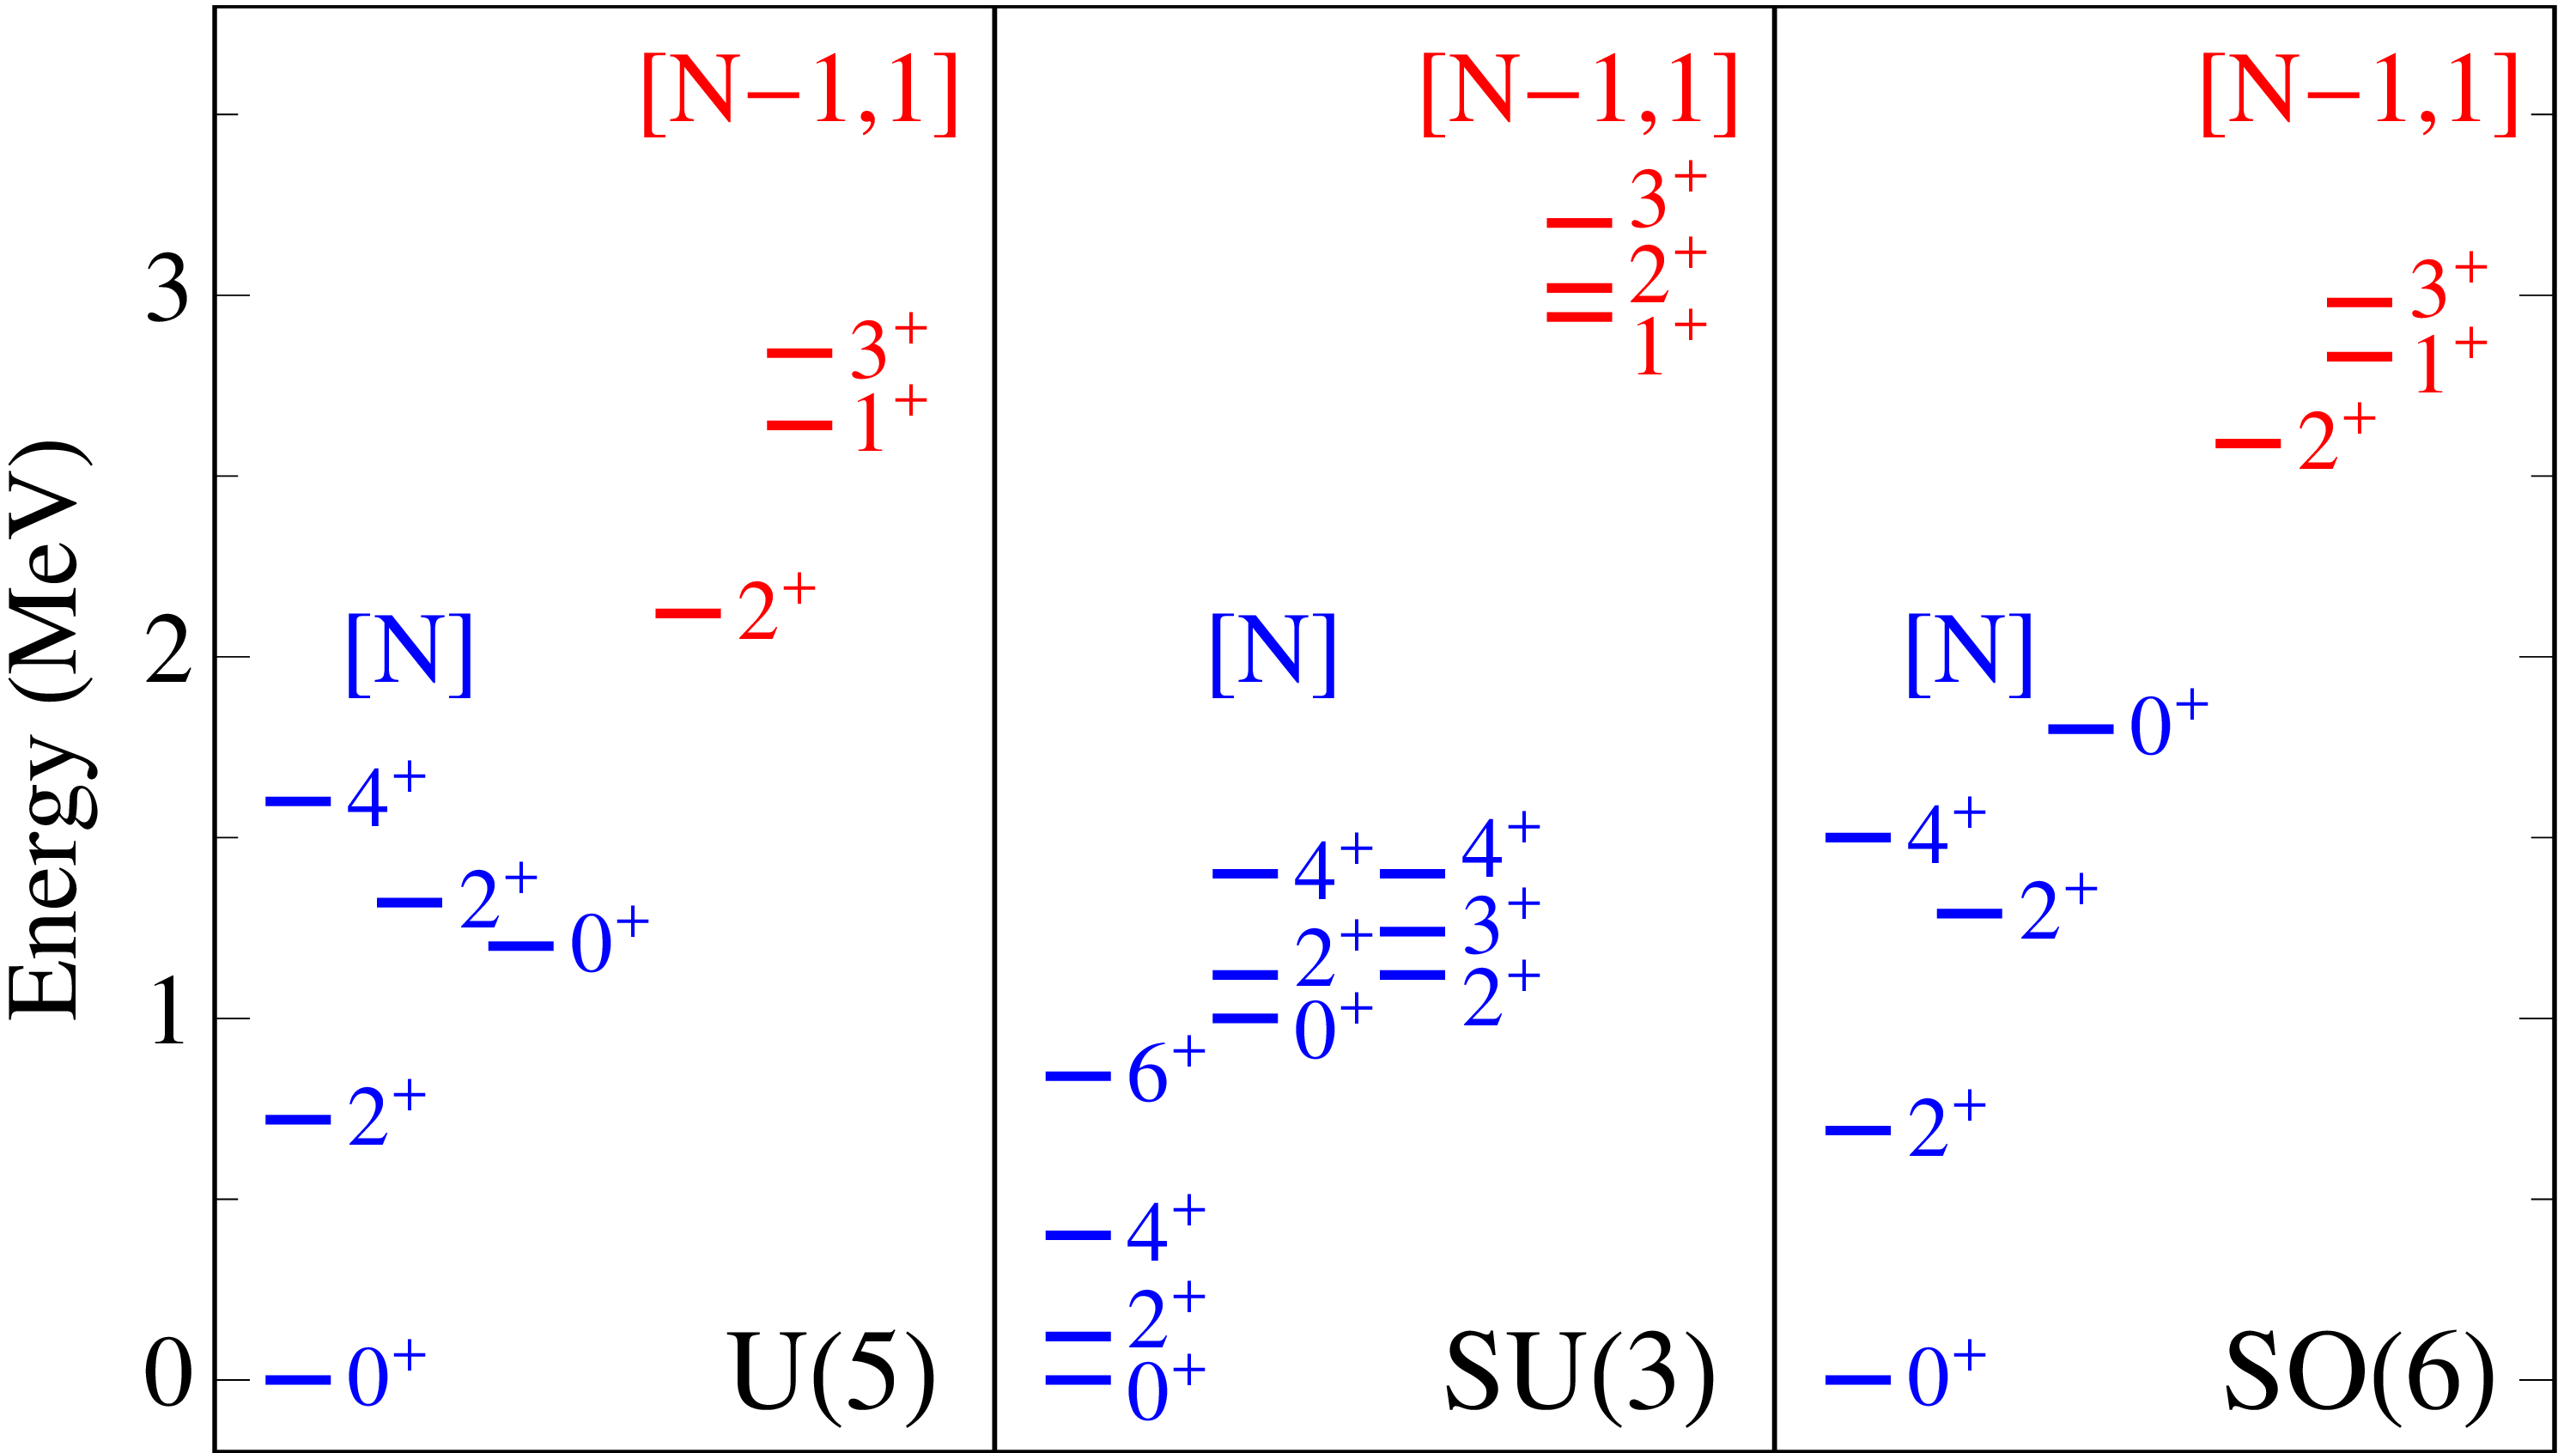
\includegraphics[width=0.6\textwidth]{figure/F_ms.png}
\caption{$F$自旋是守恒的量子数的 IBM-2 的3种极限的情况的部分能谱。能级由它们的角动量和宇称标记,$J^\pi$;还给出了U(6)的标签$[N-f,f]$。在U(6)中对称的态标记为蓝色,混合对称的态由红色表示。\label{fig_ms}}
\end{figure}


这些具有混合对称性的态的存在,在各种反应中被激发,现在已经很好地建立了。最低对称和混合对称状态的能级如图\ref{fig_ms}所示。特别相关的是$1^+$态,因为这些态在IBM-2中是允许的,但在IBM-1中是不允许的。$1^+$能级的特征激发为磁偶极型,IBM-2预测的$1^+$混合对称态的${\rm M_1}$强度为
\begin{equation*}
B({\rm M}1;0^+_1\rightarrow1^+_{\rm MS})=
{3\over{4\pi}}(g_\nu-g_\pi)^2f(N)N_\nu N_\pi,
\end{equation*}
其中$g_\nu$和$g_\pi$是玻色子的$g$因子。函数$f(N)$在IBM-2的三个主要极限中是解析已知的$f(N)=0</math>, <math>8/(2N-1)$和$3/(N+1)$,分别在U(5),SU(3)和SO(6)中。这给出了一个简单且合理准确的估算,即偶偶核中$1^+$混合对称态轨道性质的${\rm M_1}$总强度。

利用大玻色子数的极限可以找到混合对称态的几何解释。从这一分析可以看出,它们对应于中子和质子不同相的振荡,而不是对称的IBM-2态,这种振荡是同相的。这种状态的出现首先是在振动和变形核中的几何双流体模型的背景下预测的,在这种模型中,它们表现为中子-质子反振荡。由于这种几何解释,混合对称态常被称为剪刀态,这是在变形核的情况下的图像。IBM-2证实了这些几何描述,但同时还将其推广到所有原子核,不仅是球形和形变核,还有γ不稳定和过渡核。

\subsection{Neutrons and protons: Isospin}

如果中子和质子占据不同的价壳层,自然只考虑中子-中子和质子-质子对,并明确地包括这两类对之间的中子-质子相互作用。如果中子和质子占据相同的价壳层,这种方法不再有效,因为没有理由不包括$T=1$中子-质子对。接下来由 Elliott 和 White 提出的模型称为 \textbf{IBM-3}。 因为包含了完整的$T=1$的三重态,所以可以使它保持同位旋不变,从而可以与壳模型进行更直接的比较。

在IBM-3中有三种玻色子$(\nu,\delta,\pi)$,每种玻色子有六个分量,因此$N_{\rm b}$玻色子态属于U(18)的对称不可约表示。构造出具有好的总角动量$J$和良好的总同位旋$T$的IBM-3态是有可能的。

动力学的对称性的分类比较复杂,其分析还不完全。参考文献详细研究了具有动力学的U(6)对称性[或SU(3)电荷对称性]的情况。在参考文献中提出并分析了其他$J$和$T$守恒[但电荷SU(3)不守恒]的分类。IBM-3中包含的所有玻色子有$T=1$,原则上还有可以引入对应于$T=0$的中子-质子对的其他玻色子。这个进一步扩展的模型被称为IBM-4,可以被认为是IBM最精细的版本。有几个原因认为还应该包括$T=0$玻色子。在核壳模型的$LS-$耦合极限中发现了一个理由,其中最低能量的两粒子态具有轨道角动量$L=0$和$L=2$,且$(S,T)=(0,1)$或$(1,0)$。此外,在IBM-4中玻色子的选择允许包含 Wigner 超多重代数SU(4)的玻色子分类。这些有利于IBM-4的定性论据已被偶偶的和奇奇的$sd$壳核的定量、微观研究所证实。

可以说,扩展版IBM-3和IBM-4最重要的优点是,它们允许在IBM中用在壳模型中有其对应体(同位旋、Wigner 超多重态标记等等)的量子数构造动力学的对称性,而量子数在shell模型中有对应的量子数。正如 Elliott 经常强调的,这个特性允许根据壳模型检验IBM的有效性。

\subsection{Supersymmetry}

对称性技术可以应用于相互作用玻色子系统和相互作用费米子系统。在这两种情况下动力学代数都是${\rm U(\Omega)}$,${\rm \Omega}$是单粒子的允许的态的数目。在这两种情况下,都可以通过研究${\rm U(\Omega)}$的子代数来构造可解模型。毫不奇怪,同样的对称性技巧可以应用于由相互作用的玻色子和费米子组成的系统。如果玻色子和费米子对易,玻色子-费米子系统的动力学代数是${\rm U^B(\Omega_b)\otimes U^F(\Omega_f)}$,对其子代数的研究又得到了可解哈密顿量。

这个想法被应用在相互作用玻色子-费米子模型(IBFM)的中,IBFM提出了一种通过将费米子耦合到玻色子核芯来描述奇质量核的方法。偶偶和奇质量核的性质分别可以从IBM和IBFM中得到,但动力学代数${\rm U^B(6)\otimes U^F(\Omega)}$并没有得到统一的描述,它的单个的不可约表示中不同时包含两种类型的核。核超对称提供了一个理论框架,其中玻色子和费米子系统被视为同一个超多重态的成员,并且不同核的激发谱来自一个哈密顿量。这种方法成功的一个必要条件是玻色子和费米子激发能的能量标度是可比拟的,这在原子核中确实如此。原子核超对称性最初是由 Iachallo 和他的同事假设为双重态之间的对称性,随后扩展到包括奇奇核在内的原子核的四重态。

简而言之,奇奇核和奇质量核中的态的连接是由生成元
\begin{equation*}
	\left(\begin{array}{c|c}
	b^\dagger b&0\\
	---&---\\
	0&a^\dagger a
	\end{array}\right)
\end{equation*}
其中a(b)指费米子(玻色子),为了简单起见,省略了指表。偶偶核中的态由左上角的算符连接,而奇数质量核中的态则需要这两组算符。没有算符来连接偶偶核和奇质量核的态。这个代数结构的一个扩展考虑了将玻色子转换为费米子的(或反之)额外的算符,
\begin{equation*}
\left(\begin{array}
{c|c}
b^\dagger b&b^\dagger a\\
---&---\\
a^\dagger b&a^\dagger a
\end{array}
\right)
\end{equation*}
这个集合不再形成一个经典李代数,它是根据交换关系定义的。例如
\begin{equation*}
[a^\dagger b,b^\dagger a]=
a^\dagger bb^\dagger a-b^\dagger aa^\dagger b=
a^\dagger a-b^\dagger b+2b^\dagger ba^\dagger a
\end{equation*}
它们不接近原来的集合$\{a^\dagger a,b^\dagger b,a^\dagger b,b^\dagger a\}$。交叉项的包含并没有导致经典的李代数,因为双线性算子$b\dag a$和$a\dag b$的行为不像玻色子而是费米子,而$a\dag a$和$b\dag b$都具有玻色子性质。在后一个算子和对易子之间考虑反对易子可以保持封闭性。这样得到的分类或超代数是${\rm U(6/\Omega)}$,其中6和${\rm \Omega}$是玻色子和费米子代数的维数。

将${\rm U}^{\rm B}(6)\otimes{\rm U}^{\rm F}(\Omega)$嵌入到超代数${\rm U}(6/\Omega)$中,实现了偶偶核和奇质量核的统一描述。从形式上看,这可以从约化中看出
\begin{equation*}
\begin{array}{ccccc}
{\rm U}(6/\Omega)&\supset&
{\rm U}^{\rm B}(6)&\otimes&{\rm U}^{\rm F}(\Omega)\\
\downarrow&&\downarrow&&\downarrow\\[0mm]
[{\cal N}\}&&[N_{\rm b}]&&[1^{N_{\rm f}}]
\end{array}
\end{equation*}
${\rm U(6/\Omega)}$的超对称不可约表示$[{\cal N}\}$使得在玻色子中是对称的,在费米子中是反对称的,并且包含了${\rm U^B(6)\otimes U^F(\Omega)}$的${\cal N}=N_{\rm b}+N_{\rm f}$的不可约表示$[N_{\rm b}]\times[1^{N_{\rm f}}]$。因此一个单个的超对称不可约表示既包含偶偶核($N_{\rm f}=0$)的态,也包含奇质量核($N_{\rm f}=1$)的态。

最后,如果区分了中子和质子,那么自然会提出一个一般的动力学代数${\rm U}_\nu(6/\Omega_\nu)\otimes{\rm U}_\pi(6/\Omega_\pi)$,其中$\Omega_\nu$和$\Omega_\pi$分别是质子和中子的单粒子空间的维数。这个代数包含了将玻色子转换成费米子的生成元,反之亦然,而且对于中子和质子来说是不同的。现在,超多重态包含原子核的四重态(偶偶核、偶奇核、奇偶核和奇奇核),这些原子核可以用一个哈密顿量同时描述。${\rm U}_\nu(6/12)\otimes{\rm U}_\pi(6/4)$的预言已经广泛的应用于铂(platinum $Z=78$)和金($Z=79$)核的研究中,它们的中子的主要轨道是$3p_{1/2},3p_{3/2},2f_{5/2}$,质子的主要轨道是$2d_{3/2}$。探索四重态中奇奇核的性质被证明是一个挑战,并且花了许多年的专门实验来建立一个令人信服的完整的超多重态的例子,其展示在了图\ref{F_quartet_pt}和图\ref{F_quartet_au}中
\begin{figure}[H]
\centering
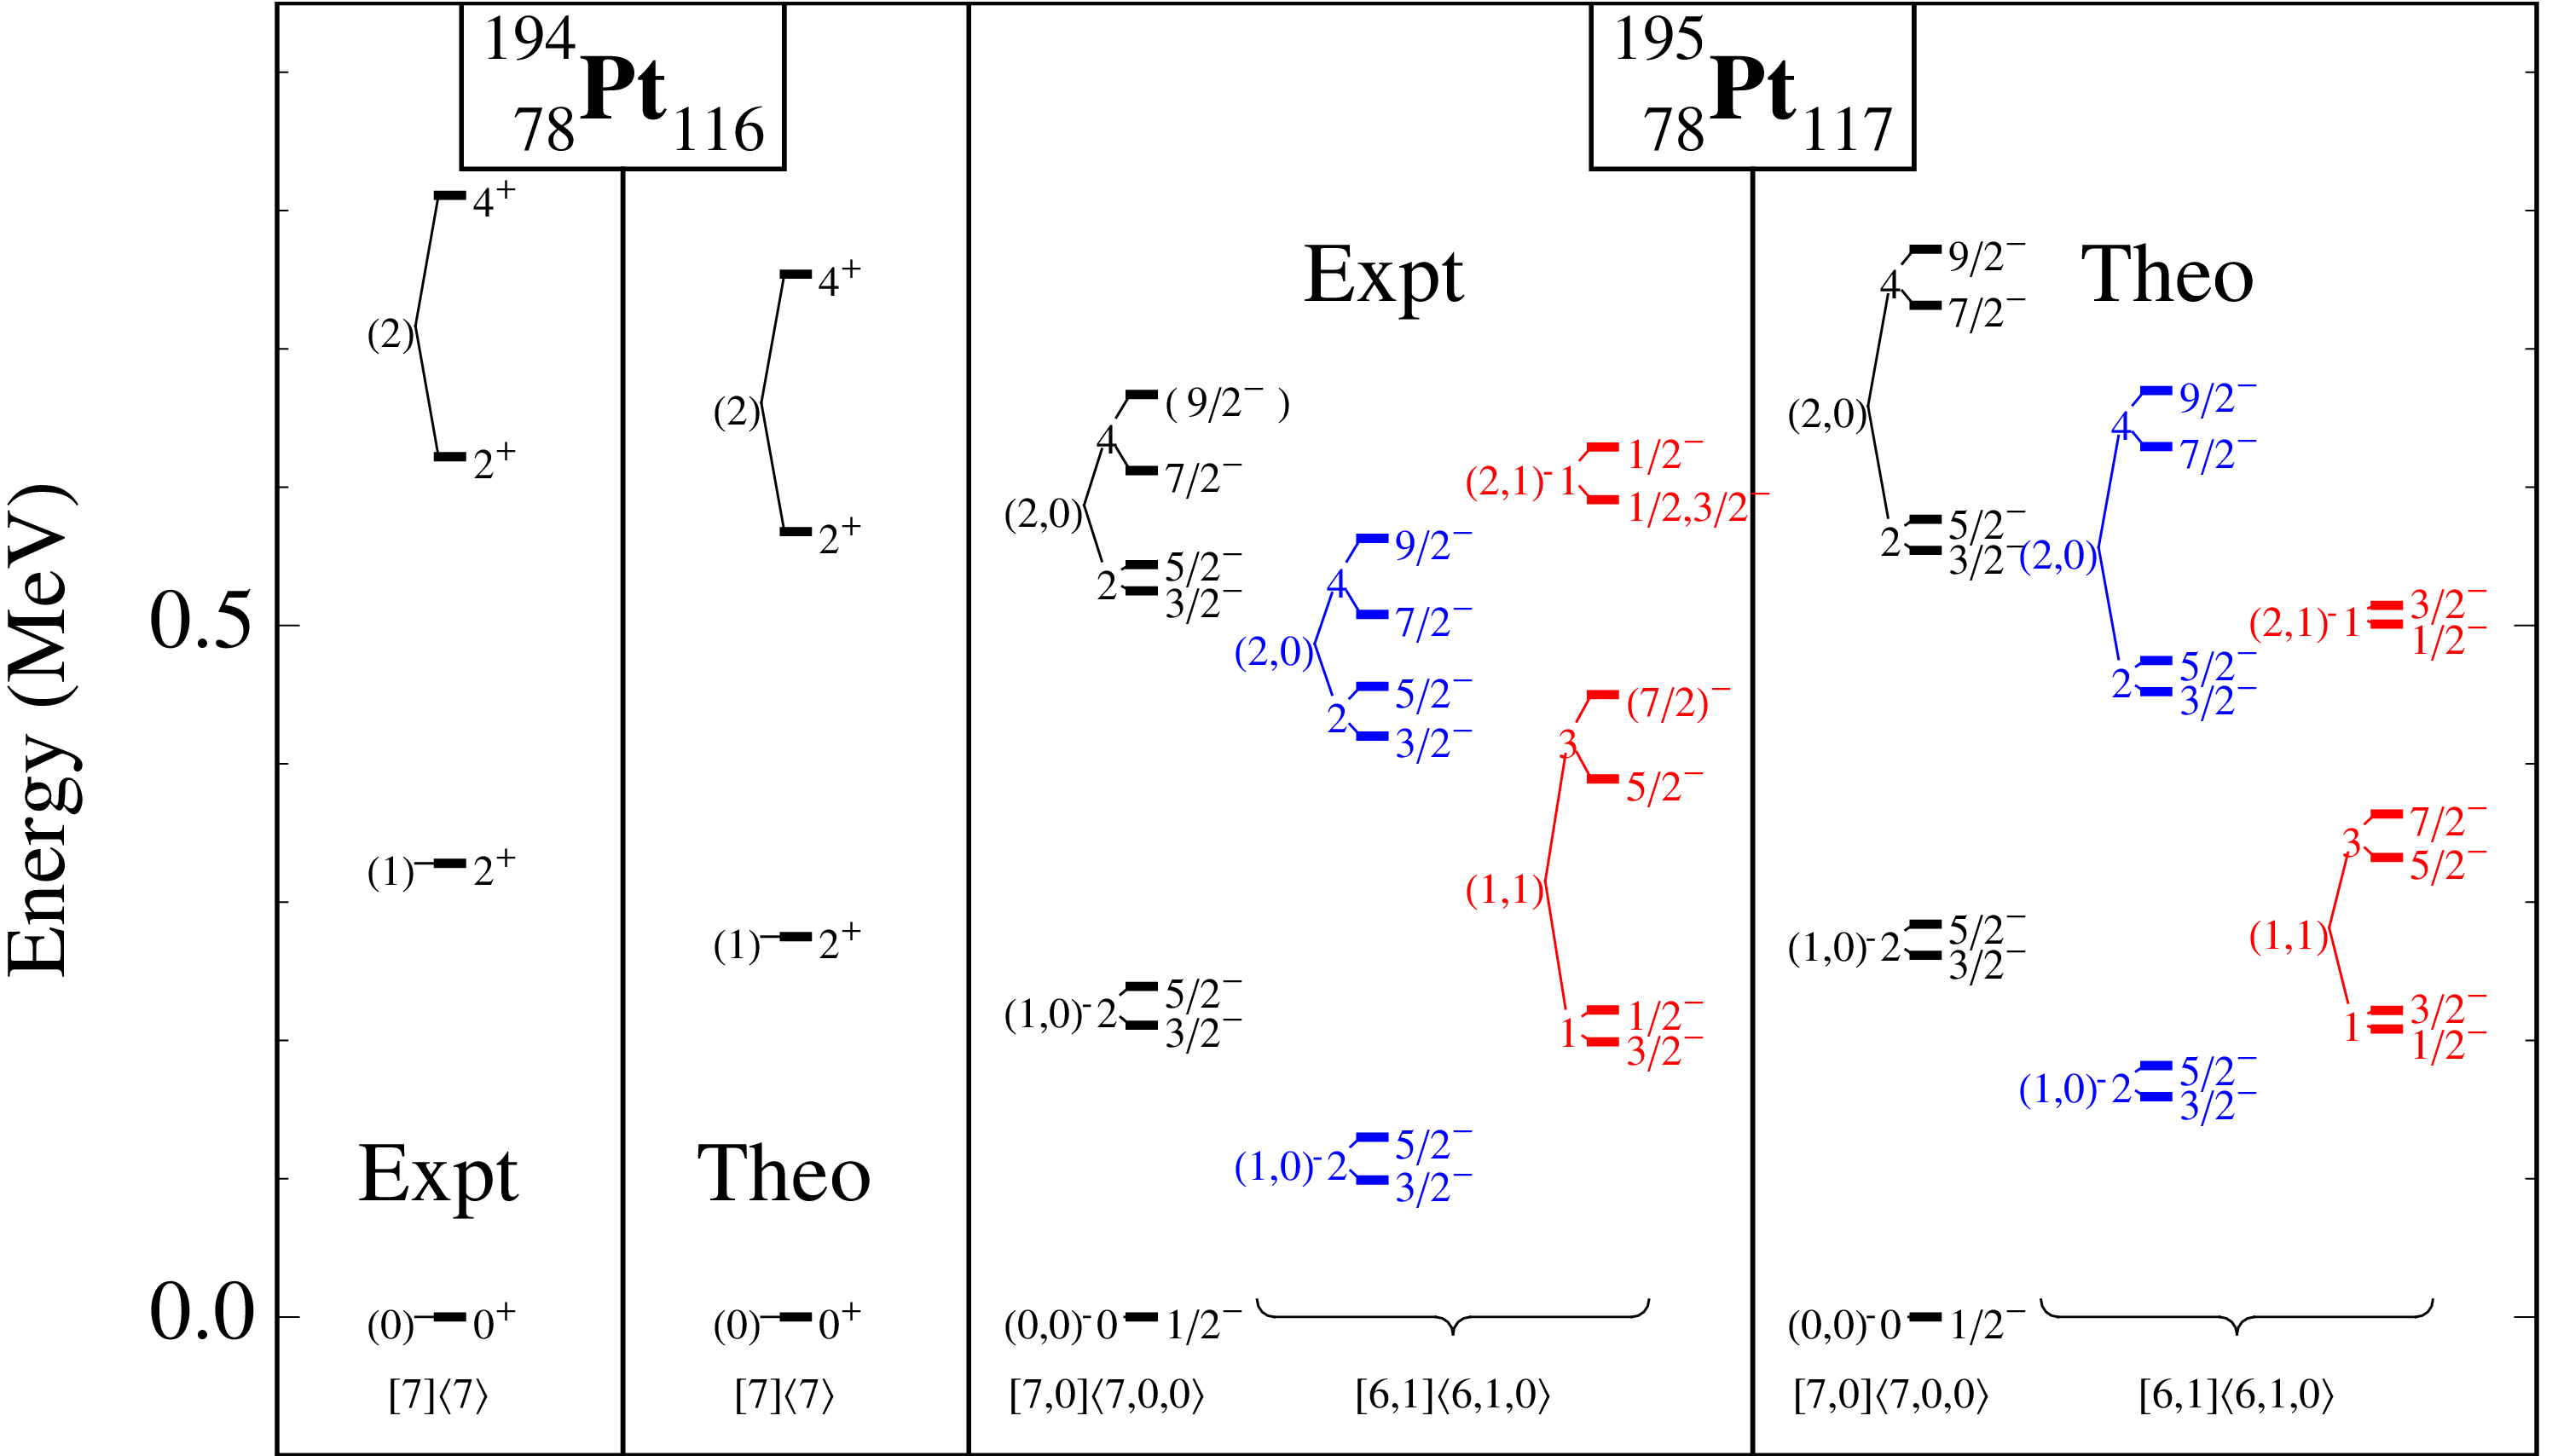
\includegraphics[width=0.6\textwidth]{figure/F_quartet_pt.png}
\caption{铂(platinum)的${\rm U}_\nu(6/\Omega_\nu)\otimes{\rm U}_\pi(6/\Omega_\pi)$超多重态成员。\label{F_quartet_pt}}
\end{figure}
\begin{figure}[H]
\centering
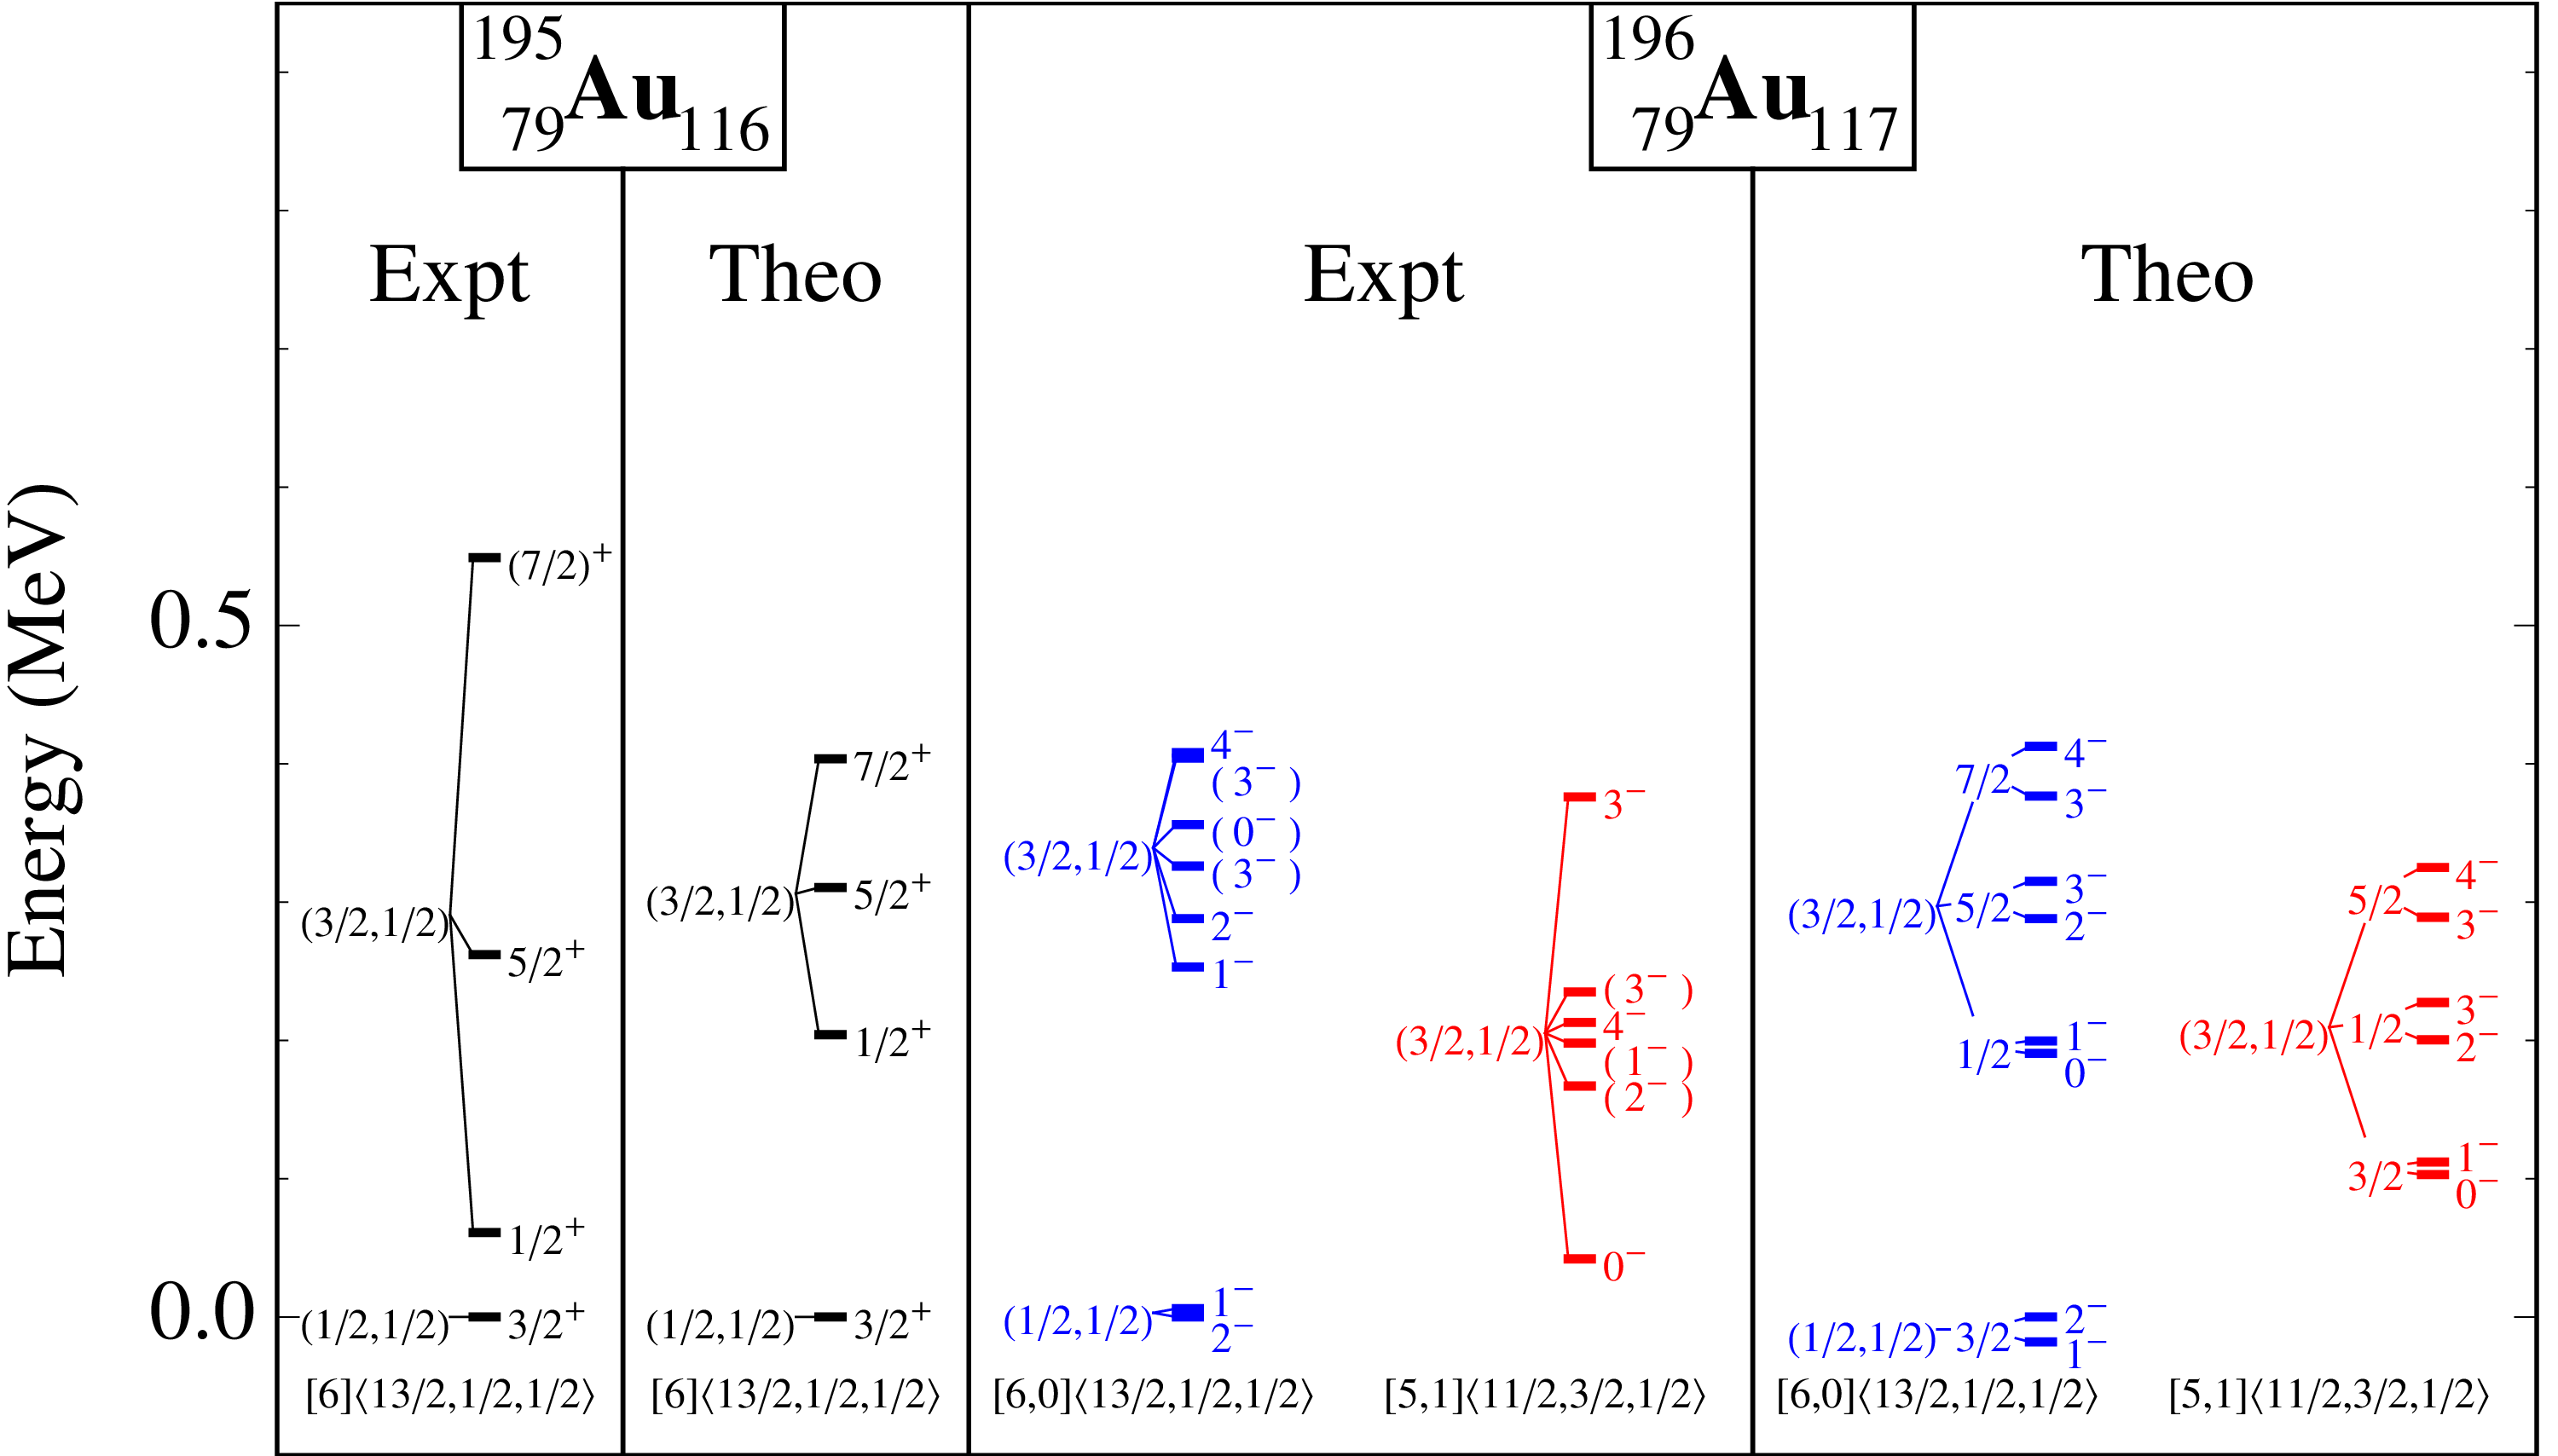
\includegraphics[width=0.6\textwidth]{figure/F_quartet_au.png}
\caption{金的${\rm U}_\nu(6/\Omega_\nu)\otimes{\rm U}_\pi(6/\Omega_\pi)$超多重态成员。\label{F_quartet_au}}
\end{figure}

\section{Beyond exact solvability}

这篇综述的讨论仅限于原子核壳模型、几何集体模型和相互作用玻色子模型的特定的哈密顿量的精确解。这一结论部分包含了对不是对所有本征态都可精确解的,而只是只对其一个子集可解的模型哈密顿量的简洁和定性的讨论。众所周知,量子力学中只有有限数量的势是解析可解的,这意味着本征值的整个能谱和相应的本征函数可以作为精确解得到。构造更广泛的一类势,对于有限(或可能无限)部分但不是整个特征值谱可以有精确解的。具有这种势的模型称为准精确可解模型(QES)。这是一个多年来一直在研究的丰富的研究领域。到目前为止,QES在核结构中的应用很少,其中一个被引入到玻尔哈密顿量体系中。

一个相关的推广涉及动力学对称性。在描述复杂的量子多体系统时,动力学对称性的条件很少被满足。一个更真实的描述需要通过在一个特定的子代数链中添加来自不同链的一个或多个项来打破动力学对称性。这通常会导致精确可解性的丧失。然而,可以构造具有部分动力对称性(PDS)的哈密顿量,使得其本征态的子集可以由特定动力学对称性的标记的子集来表征。综述(Leviatan, 2011)中对一般机制进行了精确和广泛的讨论。存在三种类型的PDS,取决于是否所有(或部分)本征态携带全部(或部分)与动力学对称性相关的量子数。

许多原子核可以被描述为在两个动力学对称性之间有一个转变(例如,在IBM中,从${\rm U(5)}$到${\rm SU(3)}$,或从${\rm U(5)}$到${\rm O(6)}$,或从配对的${\rm SU(5)}$到转动的${\rm SU(3)}$)。虽然过渡哈密顿量一般不具有动力学对称性,但结果表明,除了在过渡点之前(或之后)有一个非常窄的区域外,初始(或最终)对称性以某种有效的方式保持不变。这是可能的,因为存在准动态对称(QDS),使用嵌入表示的概念以精确的方式来表达。严格地说,具有QDS的哈密顿量是不完全可解的。然而,QDS的概念显然来源于动力学对称性,在原子核和更一般的系统的研究中有着广泛的应用。

\section{Further reading}

几乎80年的科学研究很难用30页来概括,因此,本篇综述只对大多数发展进行了短暂的讨论。因此,以一份以供进一步阅读的建议清单结束是适当的。存在许多关于物理学中的对称性和群论的书。一本标准的专著是(Hamermesh, 1962);一本最近的专著是(Iachhello, 2006)。全面介绍了核结构的标准专著是(Bohr \& Mottelson, 1969, Bohr \& Mottelson, 1975),并在(Ring \& Schuck, 1980)中讨论了该领域中使用的多体问题的技巧。有关shell模型的详细信息可以在参考文献(Heyde, 1990; Talmi, 1993)中找到,而相互作用的玻色子模型则可以在参考文献(Talmi, 1993, Iachallo \& Arima, 1987, Iachallo Van Isacker, 1991)中找到。专著(Frank, Jolie, \& Van Isacker, 2009)中概述了在描述原子核时遇到的对称性。最后,关于在壳模型框架中嵌入代数集体模型的讨论可以在书(Rowe \& Wood, 2010)中找到。

\section{Acknowledgement}

作者希望感谢 Stijn de Baerdemacker,他对本综述中涉及的几个主题进行了启发性的讨论。